\documentclass[a5paper,papersize]{corona-a5}

\usepackage{hyperref}
%\usepackage{xcolor}
\usepackage[dvipsnames]{xcolor}
\usepackage[dvipdfmx]{graphicx}
%\usepackage[dvipdfmx]{graphicx}
\usepackage{amsmath}
\usepackage{amssymb}
\usepackage{ascmac}
\usepackage{type1cm}
\usepackage{multicol}
\usepackage{makeidx}



\newcommand{\AmSLaTeX}{\leavevmode\hbox{$\mathcal A\kern-.2em\lower.376ex%
        \hbox{$\mathcal M$}\kern-.2em\mathcal S$-\LaTeX}}
\newcommand{\sibun}{\hspace{0.25zw}}

\makeindex
\begin{document}

\tableofcontents
\begin{preface}{2024年10月}{松野裕, 高井利憲, 岡本圭史}
本書は安全分析、モデルベースシステムズエンジニアリング、アシュアランスケースを解説した本です。
自動運転やドローンシステム、さらには急激に発展している生成AI技術を用いたシステムなど、
世界を変えうるシステムが登場しようとしています。




\end{preface}

\newpage
\mbox{}\thispagestyle{empty}
\clearpage

\chapter{イントロダクション}
\label{chap1}

\section{システムのディペンダビリティ:基礎概念と現代的課題}

\subsection{システムとは何か}

私たちの日常生活において、「システム」という言葉をよく耳にします。しかし、この概念を正確に定義するのは簡単ではありません。システム工学の観点から見ると、システムとは「私たちの身の回りにある、何らかのサービスを提供する物や人を抽象化した概念」と定義できます。

システムは常に特定の環境に置かれており、その環境との相互作用を通じて機能します。例えば、自動車というシステムは道路という環境の中で機能し、気象条件や交通状況などの環境要因の影響を受けます。

システムが提供する「サービス」とは、システムによって私たちに提供される機能や便益のことを指します。私たちユーザーは、このサービスを通じてシステムと関係を持ちます。例えば、スマートフォンというシステムは、通話、メッセージング、インターネット閲覧などのサービスを提供し、私たちはこれらのサービスを通じてスマートフォンと関わっています。

\subsection{ディペンダビリティの概念}

ディペンダビリティ(Dependability)は、直訳すると「依存可能性」となりますが、システム工学では「総合信頼性」と訳されることが多い重要な概念です。この概念の起源は、あるシステムが別のシステムに依存(Depend)することができる、そのシステムの性質を表すことにあります。

例えば、運転手(システムA)が自動車(システムB)に依存する場合を考えてみましょう。自動車がディペンダブル(依存可能)であるためには、どのような性質を持つべきでしょうか?安全であること、運転しやすいこと、目的地まで確実に到達できることなどが挙げられるでしょう。このように、ディペンダビリティは利用者や環境によって求められる性質が異なる、相対的な概念です。

システムがディペンダブルであるためには、以下の条件を満たす必要があります:

\begin{itemize}
\item 利用者や環境において望まれる性質を持ち続けること
\item サービスを継続的に提供すること
\end{itemize}

さらに、システムがその性質を失った場合(つまり、ディペンダブルでなくなった場合)には、速やかに復旧を行い、サービスを継続する能力も求められます。

\section{ディペンダビリティの体系と用語}

ディペンダビリティの概念は、1980年代から国際的な研究グループ(IFIP WG 10.4 "Dependable Computing and Fault Tolerance"など)によって体系化され、用語の整理が行われてきました。当初は「耐故障性(Fault Tolerance)」研究から発展し、近年ではセキュリティの概念も含めて議論されています。

ここでは、Avizienis et al. (2004)による体系に基づいて、ディペンダビリティの主要な概念を紹介します。

\subsection{ディペンダビリティ属性}

ディペンダビリティ属性は、システムがディペンダブルであるために持つべき特性を表します。主な属性には以下のものがあります:

\begin{itemize}
\item 可用性(Availability):正しいサービスの即応性
\item 信頼性(Reliability):正しいサービスの継続性
\item 安全性(Safety):利用者と環境へ破壊的影響をもたらさないこと
\item 一貫性(Integrity):不適切なシステム変更がないこと
\item 保守性(Maintainability):変更と修理を受け入れられること
\end{itemize}

これらの属性は相互に関連しており、時には相反する関係にあることもあります。システム設計者は、対象システムの要求に応じてこれらの属性のバランスを取る必要があります。

\subsection{ディペンダビリティへの脅威}

システムのディペンダビリティを脅かす要因は、以下の3つの概念で整理されています:

\begin{itemize}
\item 欠陥(Fault):エラーの原因となるとみなされる、あるいは推定されるもの、こと
\item 誤り(Error):障害が起こりうるシステムの状態(ただし、エラー状態になったからといって、必ずしも障害が起こるとは限らない)
\item 障害(Failure):サービスが正しいサービスから逸脱する出来事
\end{itemize}

これらの概念は因果関係にあり、欠陥がエラーを引き起こし、エラーが障害につながる可能性があります。

\subsection{ディペンダビリティへの脅威に対処する手段}

ディペンダビリティへの脅威に対処するため、以下の4つの手段が提案されています:
\begin{itemize}
\item 欠陥防止(Fault Prevention):欠陥の導入や発生を防ぐ
\item 耐故障性(Fault Tolerance):欠陥がある中で障害を防ぐ
\item 欠陥除去(Fault Removal):欠陥の数や深刻度を減らす
\item 欠陥予測(Fault Forecasting):欠陥の現在の数、今後の障害、影響などを予測する
\end{itemize}
これらの手段を適切に組み合わせることで、システムのディペンダビリティを向上させることができます。

\section{現代のシステムとディペンダビリティの課題}

\subsection{情報システムの規模拡大とネットワーク化}

近年、情報システムは急速に規模を拡大し、ネットワーク化が進んでいます。この変化は以下のような段階を経ています:

\begin{itemize}
\item 単機能システム
\item 複合機能システム
\item ネットワーク化されたシステム
\item サービスポータル化されたシステム
\end{itemize}

この変化に伴い、ITシステムは生活・社会インフラとしての役割を担うようになり、組込みシステムもポータル化が進んでいます。これにより、システムの複雑さと重要性が増大し、ディペンダビリティの確保がより困難かつ重要になっています。

\subsection{大規模なシステム障害のリスク}

システムの大規模化と複雑化に伴い、以下のような要因により大規模なシステム障害のリスクが高まっています:
\begin{itemize}
\item プログラムサイズの増大と多機能化
\item ブラックボックス化したコンポーネントの増加
\item 技術進化のスピードの加速
\item 接続システムの多様化
\item 利害関係者の変化と要求の頻繁な変更
\end{itemize}

これらの要因により、システムの完全な理解と制御が困難になっています。

\subsection{オープンシステム(開放系)の問題}

現代のシステムは、複雑化、ネットワーク化し、そのためそのシステムのステークホルダーの誰もが
\begin{itemize}
\item 仕様/実装の不完全さ:要求、仕様、設計、実装、テストの各段階での不完全さが避けられない
\item システムの完全理解の困難さ:構成要素の論理的不透明さ(複雑化、巨大化、ブラックボックス化)により、システム全体の挙動予測が困難
\item 使用環境の変化に伴う不確実さ:要求事項・レベルの変化、想定外の使われ方、ネットワークを介しての構成要素の変化
\item セキュリティリスクの増大:ネットワークを介した外部からの意図的な攻撃のリスク
\end{itemize}

\section{これからのディペンダビリティに向けて}

\subsection{不完全・不確実なシステムへの対応}

従来の形式手法やテストなどの手法に加え、不完全・不確実なシステムがディペンダブルであるための新たなアプローチが必要とされています。しかし、完全に障害を排除することは不可能であり、深刻な障害が起こる可能性は以前よりも高まっています。

\subsection{システム保証(System Assurance)の重要性}

このような状況下で重要になってくるのが「システム保証」の概念です。システム保証とは、システムがどの程度ディペンダブルか、あるいはディペンダブルでないか、リスク分析などをもとに利用者などのステークホルダーに説明し、納得してもらうプロセスです。

絶対に安全である、あるいは完全にディペンダブルであることは不可能であるという事実を、ステークホルダーに理解してもらうことが重要です。

\subsection{説明責任の必要性の高まり}

近年、システムの安全性や信頼性に関する説明責任の重要性が高まっています。例えば、2009-2010年のトヨタ プリウスの北米大規模リコール問題では、原因説明への準備不足が指摘されました。

また、自動車の機能安全規格であるISO 26262の制定により、自動車メーカーはより説明しやすい形で安全性の根拠を示すことが求められるようになりました。

\subsection{AI技術とディペンダビリティ}

最近では、AI(人工知能)技術を用いたシステム、特に自動運転システムなどのディペンダビリティが重要な課題となっています。AI技術の不確実性や説明可能性の問題は、従来のシステムとは異なる新たなディペンダビリティの課題を提起しています。


システムのディペンダビリティは、もはや単なる技術的な問題ではなく、社会的、倫理的な問題としても捉えられるようになっています。システムの複雑化、不確実性の増大、そしてAI技術の台頭により、従来のディペンダビリティの概念や手法だけでは不十分になってきています。

これからのディペンダビリティ確保には、技術的な対策に加えて、システム保証と説明責任の遂行が不可欠です。また、不完全性や不確実性を前提としたシステム設計と運用の考え方を確立していく必要があります。

システム開発者、運用者、そして利用者を含むすべてのステークホルダーが、これらの課題を理解し、協力してディペンダブルなシステムの実現に取り組むことが求められています。
\chapter{安全分析の基本手法:FTAとFMEA}
\label{chap2}

\section{はじめに}

本書では、ディペンダビリティ(Dependability)の新しい潮流として、STAMP/STPA などの先進的安全分析手法や、システムズエンジニアリング、アシュアランスケースといった概念を取り入れ、複雑化・高度化するシステムにどう対処していくかを議論します。  
しかしながら、これらの新たなアプローチを理解・活用するにあたっても、従来から用いられてきた\textbf{既存の安全分析手法}をしっかり押さえておくことは極めて重要です。そこで本章では以下の2つの手法を紹介します。

\begin{itemize}
 \item \textbf{FTA (Fault Tree Analysis)}:  
   重大事故や障害をトップ事象とし、どのような要因の組み合わせで発生するかを論理ゲートを用いて可視化する「トップダウン型」手法。
 \item \textbf{FMEA (Failure Mode and Effects Analysis)}:  
   製品や工程の部品ごとに故障モードを洗い出し、それぞれがシステム全体に及ぼす影響を評価する「ボトムアップ型」手法。
\end{itemize}

これらはいずれも、システムや製品の\textbf{信頼性}・\textbf{安全性}を高めるうえで、長年にわたって活用されてきた「定番」の解析メソッドです。STAMP/STPA やアシュアランスケースといった新手法を導入する際にも、過去の事例や基準を踏まえたうえで、既存手法(FTA や FMEA)の成果物や解析結果を再利用したり、組み合わせたりするケースが非常に多いと考えられます。

そこで本章では、まず\textbf{FTA} を取り上げ、その基本的な進め方や利点・留意点を解説し、その後、\textbf{FMEA} の概要を示します。これらの内容は、後続の章で扱うシステムズエンジニアリングやアシュアランスケース作成、あるいは STAMP/STPA の理解を深めるための基礎にもなるでしょう。

\section{FTA (Fault Tree Analysis)}
\label{sec:FTA}

\subsection{FTA の概要と目的}

FTA は、発生してはならない重大な故障や不具合を「トップ事象」に設定し、なぜそれが起こるのかを下位に向かって論理的に掘り下げる\textbf{トップダウン型}の手法です。1979 年のスリーマイル島原子力発電所事故の解析で有効性が示されたことを契機に、原子力、自動車、航空宇宙、一般的な製造業など幅広い分野に広まっています。

\begin{itemize}
 \item \textbf{特徴}:
   \begin{itemize}
    \item 木構造(故障の木)を用いて、視覚的に「なぜ起こるか」を整理
    \item AND/OR ゲートで複数要因・並列要因を表現可能
    \item 大事故や重大障害の原因を重点的に深掘りするのに適している
   \end{itemize}
 \item \textbf{注意点}:
   \begin{itemize}
    \item トップ事象の選定を誤ると見落としが生じる
    \item システム全体の網羅的な故障モード抽出には、FMEA など他手法との併用が望ましい
   \end{itemize}
\end{itemize}

\subsection{FTA の進め方}

FTA は大きく以下の手順に従います。主に「故障の木 (FT 図) の作成」と「作成後の解析」の 2 段階です。

\begin{enumerate}
 \item \textbf{FTA 実施の準備}  
   \begin{itemize}
    \item 解析対象システムを熟知するエンジニアや品質保証担当者など、3--6 名程度のチームを編成
    \item 関連設計資料・図面・クレーム情報などを集める
   \end{itemize}

 \item \textbf{解析対象の機能の理解}  
   \begin{itemize}
    \item 対象システムの構造・機能・使用環境・周辺システムとのインタフェースを共有
   \end{itemize}

 \item \textbf{トップ事象の選定}  
   \begin{itemize}
    \item 「明確に定義できる」「発生が望ましくない」「対策可能な要因が想定される」などの観点でトップ事象を決める
    \item 例:\textbf{「エンジンが始動しない」「照明が点灯しない」「ブレーキが効かない」} など
   \end{itemize}

 \item \textbf{トップ事象の 1 次要因への展開}  
   \begin{itemize}
    \item トップ事象が起こる直接原因を OR/AND ゲート等で整理
    \item 構成要素や機能的観点から、漏れなく候補を挙げる
   \end{itemize}

 \item \textbf{トップ事象の 2 次要因以下への展開}  
   \begin{itemize}
    \item さらに「なぜそうなるのか」を繰り返し、基本事象または非展開事象に至るまで木構造を描く
    \item 要因の階層を揃え、曖昧な表現を避ける
   \end{itemize}
\end{enumerate}

\subsection{FT 図を読む:記号とゲート}

FTA では、\textbf{事象 (イベント)} を示す記号と、\textbf{論理ゲート} を使って因果関係を可視化します。

\begin{itemize}
 \item \textbf{イベント記号}:
   \begin{itemize}
    \item トップ事象(長方形)/中間事象(長方形)/基本事象(円)など
   \end{itemize}
 \item \textbf{論理ゲート}:
   \begin{itemize}
    \item AND ゲート:下位要因が「すべて発生」した場合に上位事象が成立
    \item OR ゲート:下位要因の「いずれか 1 つが発生」した場合に上位事象が成立
   \end{itemize}
\end{itemize}

\subsection{FT 図の定量的解析}

FT 図を作成したら、以下の定量解析を行う場合があります。

\begin{itemize}
 \item \textbf{トップ事象の発生確率}:
   \begin{itemize}
    \item OR ゲート $\to$ 下位事象確率の和(近似)
    \item AND ゲート $\to$ 下位事象確率の積(独立性前提)
   \end{itemize}

 \item \textbf{同一事象の排除}:
   \begin{itemize}
    \item 同じ基本事象が複数箇所に重複する際、定量計算時には一つにまとめるなど配慮が必要
   \end{itemize}

 \item \textbf{重要事象の抽出}:
   \begin{itemize}
    \item OR ゲート配下では、確率が高い事象から優先的に対策
    \item AND ゲートを含む複合形状では別の分析手段(最小カット集合など)と併用
   \end{itemize}
\end{itemize}

\subsection{FT 図の定性的解析}

発生確率の情報がない、あるいは推定困難な場合には、定性的な方法で「主要な要因」を特定することが可能です。

\begin{itemize}
 \item \textbf{最小カット集合 (Minimal Cut Sets)}:
   \begin{itemize}
    \item トップ事象を発生させる「最小限の基本事象の組み合わせ」を抽出
    \item 共通して含まれる基本事象があれば、そこを対策することでトップ事象発生を大きく防止可能
   \end{itemize}

 \item \textbf{構造重要度 (Structure Importance)}:
   \begin{itemize}
    \item ある基本事象が故障/正常化したときにトップ事象の発生パターンがどれくらい変化するかを計算
    \item トップ事象の回避への寄与度が高い基本事象を抽出する
   \end{itemize}
\end{itemize}

\subsection{FTA 実施上の留意点}

\begin{itemize}
 \item \textbf{全ての基本事象の発生確率把握は難しい}  
   \begin{itemize}
    \item 信頼性データが乏しい場合、定性的評価や他手法との併用が有効
   \end{itemize}

 \item \textbf{創発故障や相互作用に注意}  
   \begin{itemize}
    \item 単に構造分割するだけでなく、機能の流れや外部環境の影響も考慮
   \end{itemize}

 \item \textbf{動的変化を扱いにくい}  
   \begin{itemize}
    \item FTA は基本的に静的モデルであり、時間依存のリスク変化には別途検討が必要
   \end{itemize}

 \item \textbf{事後解析でも有効}  
   \begin{itemize}
    \item 実際に発生した故障・事故の原因を特定し、最小カット集合などで要因を絞る手段としても活用される
   \end{itemize}
\end{itemize}

\section{FMEA (Failure Mode and Effects Analysis)}
\label{sec:FMEA}

続いて、FMEA について簡単に紹介します。FMEA は \textbf{ボトムアップ型} で故障モードを分析する手法であり、FTA と組み合わせることで、システム全体の安全分析をより強固にする狙いがあります。  
本書では後の章で扱う STAMP/STPA やアシュアランスケースとも対比しながら、従来手法との使い分け・組み合わせを検討します。

\subsection{FMEA の概要と目的}

\begin{itemize}
 \item 故障モード (Failure Mode) を部品・工程レベルから列挙し、それが上位システムへ及ぼす影響 (Effects) を評価する未然防止手法
 \item NASA での宇宙開発プロジェクトや自動車、家電、医療機器など多様な領域で実績がある
\end{itemize}

\subsection{FMEA の進め方 (概略)}

\begin{enumerate}
 \item \textbf{準備とチーム編成}
 \item \textbf{解析対象の機能・構造把握}
 \item \textbf{故障モードの抽出}
 \item \textbf{影響評価 (Severity / Occurrence / Detection) と優先度 (RPN)}
 \item \textbf{対策検討とフォローアップ}
\end{enumerate}

\subsection{FMEA の利用事例とまとめ}

\begin{itemize}
 \item \textbf{工程 FMEA}:製造工程や組立工程における不良モードを系統的に洗い出す
 \item \textbf{設計 FMEA}:製品の詳細設計時に、部品・サブシステムの故障モードを網羅し、上位への影響を検討
 \item これらの\textbf{FMEA} と \textbf{FTA} を組み合わせることで、網羅性(FMEA)と重大事象の重点把握(FTA)が両立できる
\end{itemize}

% end of chapter


\chapter{安全分析手法STAMP/STPA}
%岡本さん
\label{chap3}



\section{STAMP(System-Theoretic Accident Model and Processes)の概要}

% pp.6-8の「背景」は(今は)書かないことにする。
STAMP(System-Theoretic Accident Model and Processes)は、システム理論に基づく新しい事故モデル(Accident Model)である。従来の事故モデルが主にコンポーネントの故障(Failure)に焦点を当てているのに対し、STAMPはシステム全体の安全制約(Safety Constraint)とその制御に注目する。

\subsection{STAMPの基本概念}

STAMPの基本要素は以下の3つである: % pp.11

\begin{itemize}
    \item 安全制約:安全が守られるために必要なルール
    \item プロセスモデル:コントローラが認識するコントロール対象の状態
    \item コントロールストラクチャ:コンポーネントとそれらの間の相互作用を示したシステムの設計図
\end{itemize}

STAMPでは、アクシデントを単純なイベントの連鎖ではなく、安全制約が安全制御により適切に守られなかった結果として捉える。

\section{STPA(System-Theoretic Process Analysis)}

STPAは、STAMPに基づくハザード分析手法である。
システムの設計段階や運用開始前に潜在的なハザードを特定し、安全制約を導出するために使用される。

\subsection{STPAの手順}

STPAは以下の4つのステップで構成される(STPA Handbook(2018)):

\begin{enumerate}
    \item[Step 1]: 分析目的の定義
    \item[Step 2]: 制御構造図のモデル化
    \item[Step 3]: 非安全制御動作の識別
    \item[Step 4]: ロスシナリオの識別
\end{enumerate}

以下の各項で、STPAの各ステップについて解説する。

%%%%%%%%%%%%%%%%%%%%%%%%%%%%%%%%%%%%%%%%%%%%%%%%%%%%%%%%%%%%%%%%
\subsection{Step 1: 分析目的の定義}

Step 1「分析目的の定義」では、以下を項目を実施する: %pp.27

\begin{itemize}
    \item ロス(・アクシデント)の識別
    \item システムレベルのハザードの識別
    \item システムレベルの安全制約の識別
    \item ハザードの詳細化(任意)
\end{itemize}

各用語の定義は以下のとおりである。 % pp.28

ロス(loss)は、ステークホルダにとって受容できない何かであり、
例として、人命の喪失、人の負傷、環境汚染、ミッション失敗等が挙げられる。
アクシデント(accident)は、望まれない・計画されていないイベントで、ロスへ至るものである。
例として、自車両が前方障害物に激突等が挙げられる。
以前のSTPAの解説ではアクシデントが識別されていたが、STPA Handbook(2018)では、アクシデントを識別するよう記載されていない。しかし、ロスと合わせてアクシデントを識別することで、ハザードが識別しやすくなるため、ここではアクシデントについても触れることにした。

ハザード(hazard)は、システムの状態または条件の集まりで、最悪の環境条件下で、ロスへ至る蓋然性が高いものである。
なお、ハザードはシステムの状態または条件の集まりであるため、システム境界外を直接扱わない。
例えば、「自車両が(外部環境である)前方障害物に衝突した状態」はハザードではない。
この場合、例えば「(自車両内の前方障害物検出用の)距離センサの値が規定値未満である状態」がハザードとなる。
また、ハザードは必ずしもロスへ至るわけではないことにも注意が必要である。
例えば、距離センサの値が規定値未満であったとしても、前方障害物を回避でき、人命の喪失や負傷へ至らないかもしれない。逆に「自車両が走行中である状態」は、最悪の環境下でロスへ至るが、ロスに至るまでの追加条件が多い(ロスへ至る蓋然性が低い)ため、はざーとしては扱わない。

安全制約(safety constraint)は、システムレベルの条件・動作で、ハザードを防ぐために満たす必要のあるものであり、素朴な安全制約はハザードの裏返しとして定義でき、またハザード発生時にロスを防ぐあるいは最小化する条件・動作としても定義できる。
例えば、ハザード「距離センサの値が規定値未満である状態」を防止するために、「\textcolor{red}{要検討:}自動運転システムは、距離センサの値が規定値未満になったら、自車両を安全に停止させなければならない」といった安全制約が考えられる。

ロス(・アクシデント)、ハザード、安全制約は、番号を付け、ハザードには対応するロスの番号を含める。

\subsubsection{演習:ロス、ハザード、安全制約の識別} % pp.29-35

\textcolor{red}{システムの説明を記述し、図を挿入すること。}

\begin{enumerate}
    \item 上のシステムに対するロス及びアクシデントを識別しなさい。
    (解答例:乗員の死亡・負傷(自車両が前方障害物に衝突))
    \item (i)で識別したロスに対し、ハザードを識別しなさい。
    (解答例:(前方障害物検出用の)距離センサの値が規定値未満)
    \item (ii)で識別したハザードに対し、安全制約を識別しなさい。
    (解答例1:距離センサの値が規定値未満になってはならない。解答例2:自動ブレーキシステムは、距離センサの値が規定値未満にならないよう、ブレーキを指示しなければならない。)
\end{enumerate}

%%%%%%%%%%%%%%%%%%%%%%%%%%%%%%%%%%%%%%%%%%%%%%%%%%%%%%%%%%%%%%%%
\subsection{Step 2: 安全制御構造図のモデル化}

Step 2「安全制御構造図のモデル化」では、安全制御構造図(Safety Control Structure Diagram)を構築します。
安全制御構造図(Safety Control Structure Diagram)は、システム内の構成要素(コンポーネント)間の制御関係とフィードバック関係を示すシステムのモデルで、下図(図3.1)のコントロール・ループにより構成されます。
また、コントロール・ループは以下の構成要素により構成されます。

\begin{itemize}
    \item コントローラ:制御する側のコンポーネント
    \item コントロールアルゴリズム:コントローラの判断決定プロセス、コントロールアルゴリズムに基づき、コントロールアクションを指示します。
    \item プロセスモデル:コントローラの内部情報で、判断の際に参照される情報。コントローラが認識する被コントロール・プロセスや外部環境の状態であり、プロセスモデルはフィードバックにより更新されます。
    \item 被コントロール・プロセス:制御される側のコンポーネント
    \item コントロールアクション:被コントロール・プロセスの動作や制約を実行させるための命令・指示。
    \item フィードバック:被コントロール・プロセスや外部環境の情報。
\end{itemize}

\begin{figure}[H]
    \centering
    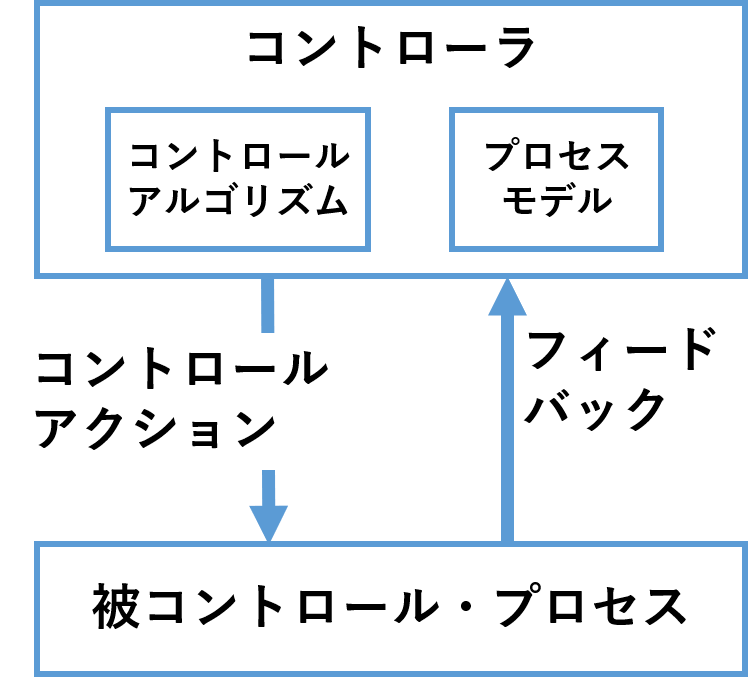
\includegraphics[width=40mm]{safety_assurance_contents/ch3images/fig-3-2-3-01.png}
    \caption[short]{コントロール・ループ}
\end{figure}

下図(図3.2)は、赤線で囲まれた二つのコントロール・ループにより構成される安全制御構造図の例です。
安全制御構造図では、制御する側を上に、制御される側を下にして記述します。
また図3.2には、アクチュエータとセンサを記載してありますが、比較的新しい文献では、
安全制御構造図を構築する際にはこれらを記載せず、後の分析(Step4)でこれらを追加して分析をするようになっています。

\begin{figure}[H]
    \centering
    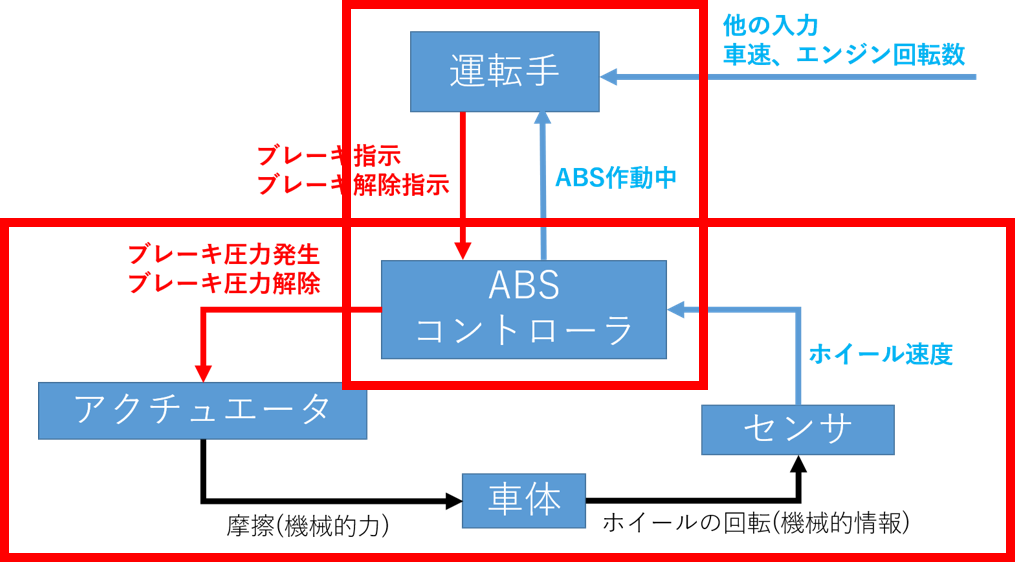
\includegraphics[width=40mm]{safety_assurance_contents/ch3images/fig-3-2-3-02.png}
    \caption[short]{例:二つのコントロール・ループにより構成される安全制御構造図}
\end{figure}

安全制御構造図は、物理的設計レベルではなく、機能レベルでのシステムのモデルです。
また、安全制御構造図はモデルですので、安全機構に関係無い機能は省略します。

安全制御構造図を基に分析することで、例えば、
センサが故障した結果、コントローラが間違ったフィードバックを受信して、
コントローラが誤った判断を下すといった事故のシナリオが識別できます。
また、プロセスモデルを考えることで、実際は自車両の前方に歩行者がいるのに、
コントローラ(自動運転車)は歩行者がいないと認識しており、その結果、事故に至るといったシナリオを分析しやすくなります。
さらに、コントローラが判断する際に必要なフィードバックが不足していたといった重大な欠陥を早期に見つけやすくなります。

機械以外にも、人間や組織をコントローラとする場合もあります。
この場合、コントロールアルゴリズムは人間の判断プロセスに、プロセスモデルは人間の認識になります。
また、(分析対象システムの外側である)外部環境からのフィードバックを考えることもあります。
例えば、自動運転車の安全制御構造図では、運転者を最上位のコントローラとし、運転者へのフィードバックとして、
目視情報(自車両の前方に歩行者がいる・いない等)を考えます。
分析の際に、安全制御構造図に人間や組織を含められるため、人間のミスや、他組織からの外圧を含めた事故のシナリオを考えられるようになります。

\subsubsection{演習:安全制御構造図の構築} % pp.44

\textcolor{red}{システムの説明を記述し、図を挿入すること。}

%% pp.52-66の「詳細化によるCSDの構築」を書くか?

%%%%%%%%%%%%%%%%%%%%%%%%%%%%%%%%%%%%%%%%%%%%%%%%%%%%%%%%%%%%%%%%
\subsection{Step 3: 非安全制御動作の識別}

Step 3「非安全制御動作の識別」では、非安全制御動作(UCA: Unsafe Control Action)を識別し、可能であればコントローラ制約を定義します。
UCAは、特定のコンテキストと最悪の環境の下で、ハザードを引き起こす可能性のある制御動作で、
コントローラ制約はUCAを引き起こさないために満たす必要のあるコントローラへの動作(制約)です。

UCAは文章として表すことが多いですが、

「制御動作を出すコントローラ」+「タイプ」+「制御動作」+「コンテキスト」+「ハザード」

の組として考えると、UCAを識別しやすくなります。
このとき、タイプとして以下の4つを用います:
%
\begin{enumerate}
    \item 与えられないとハザード
    \item 与えられるとハザード
    \item 早すぎ、遅すぎ、誤順序でハザード
    \item 早すぎる停止、長すぎる適用でハザード
\end{enumerate}
また、コンテキストは制御動作が非安全となる条件を表します。

UCAの例として、「運転者からのブレーキ指示があり、タイヤがロックしていないにもかかわらず、ABSコントローラがブレーキ圧力発生を指示しないため,前方障害物との距離が規定値未満になる.(H3)」を考えます。
コントローラ「ABSコントローラ」に対するこのUCA対するコントローラ制約として、このUCAを否定形である
「運転者からのブレーキ指示があり、タイヤがロックしていないときには、ABSコントローラがブレーキ圧力発生を指示する。」
を考えることができます。
このとき、このUCAは以下のように分解されます:
%
\begin{itemize}
    \item 制御動作を出すコントローラ:ABSコントローラ
    \item タイプ:与えない
    \item 制御動作:ブレーキ圧力発生
    \item コンテキスト:運転手からのブレーキ指示があり、タイヤがロックしていない
\end{itemize}
%
制御動作を出すコントローラ、タイプ、制御動作、ハザードは既に識別されているため、それらを組み合わせて考えることで、網羅的な分析が可能になります。
しがって、コンテキストを識別することが最も重要となります。
このとき、制御動作を出すコントローラの入力に着目すると、コンテキストが考えやすくなります。
また識別したUCAに番号を付け、以下のような表形式で表すと可読性が高まり、後の分析が容易になります。
%
\begin{figure}[H]
    \centering
    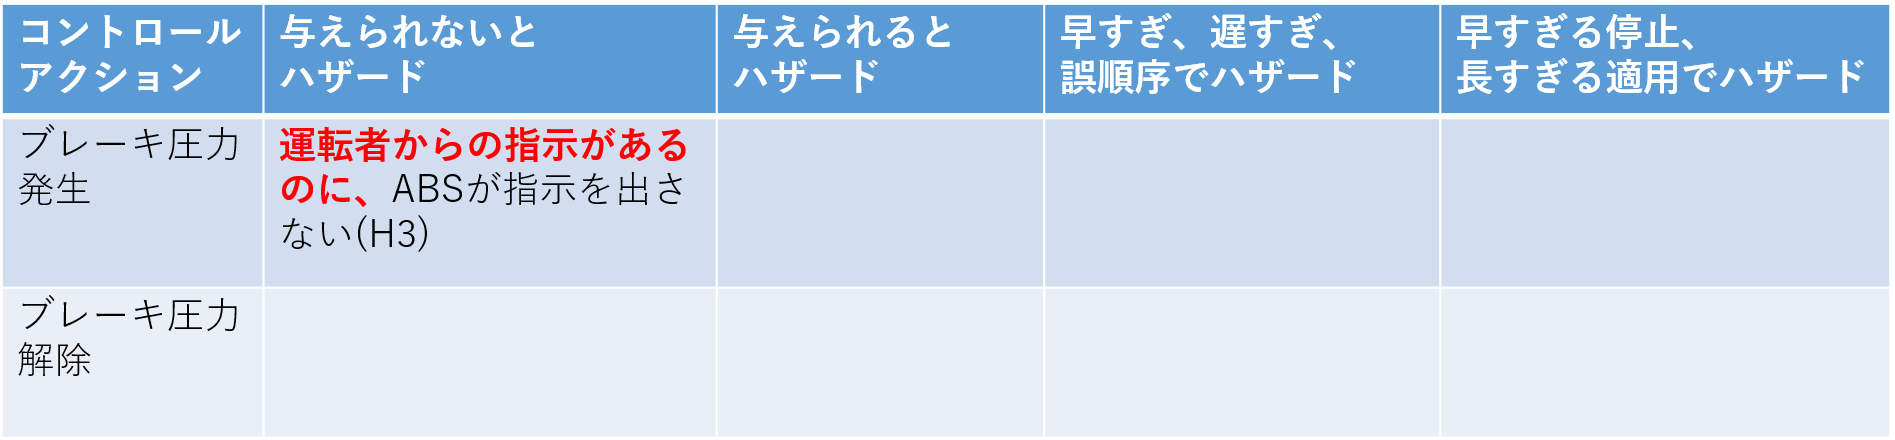
\includegraphics[width=40mm]{safety_assurance_contents/ch3images/fig-3-2-3-03.png}
    \caption[short]{例:UCAの表}
\end{figure}

コンテキストが無いにもかかわらずUCAとなる場合や、同じコンテキストの下で与えても、
与えなくてもUCAとなる場合には、その制御動作は設計には問題があると考えられます。

\subsubsection{演習:UCAの識別} % pp.74,75

\textcolor{red}{システムの説明を記述し、図を挿入すること。}

%%%%%%%%%%%%%%%%%%%%%%%%%%%%%%%%%%%%%%%%%%%%%%%%%%%%%%%%%%%%%%%%
\subsection{Step 4: ロスシナリオの識別}

\textcolor{red}{ここから再開 2024-09-17}

Step 4「ロスシナリオの識別」では、Step 3で識別したUCAに対してロスシナリオを識別します。
ロスシナリオ(Loss Scenario)は、UCA、ひいてはハザードへ至る要因を記述したシナリオです。
ロスシナリオの中で具体的要因を識別するので、アクチュエータとセンサを入れたコントロール・ループを基に分析します。

大きく分けて、以下の2種類のロスシナリオを考えます:
%
\begin{itemize}
    \item UCAへ至るシナリオ
    \item 制御動作の不実行・不適切な実行を表すシナリオ
\end{itemize}
%
「UCAへ至るシナリオ」では、図3.2.5.1の右上部分に着目し、なぜUCAが発生したのかを考えます。
UCAが発生する主な要因としては、コントローラの非安全な動作や、不適切なフィードバック・(他コントローラ等からの)入力が考えられます。 % 84ページ「コントロールループで安全制約を破られる要因の例2」の図を入れるか?
また「制御動作の不実行・不適切な実行を表すシナリオ」では、図3.2.5.1の左下部分に着目し、
なぜ制御動作は不適切に実行されたのか、なぜ制御動作は実行されなかったのかを考えます。
\textcolor{red}{さらに、86ページの説明と図を追加する。}
%
\begin{figure}[H]
    \centering
    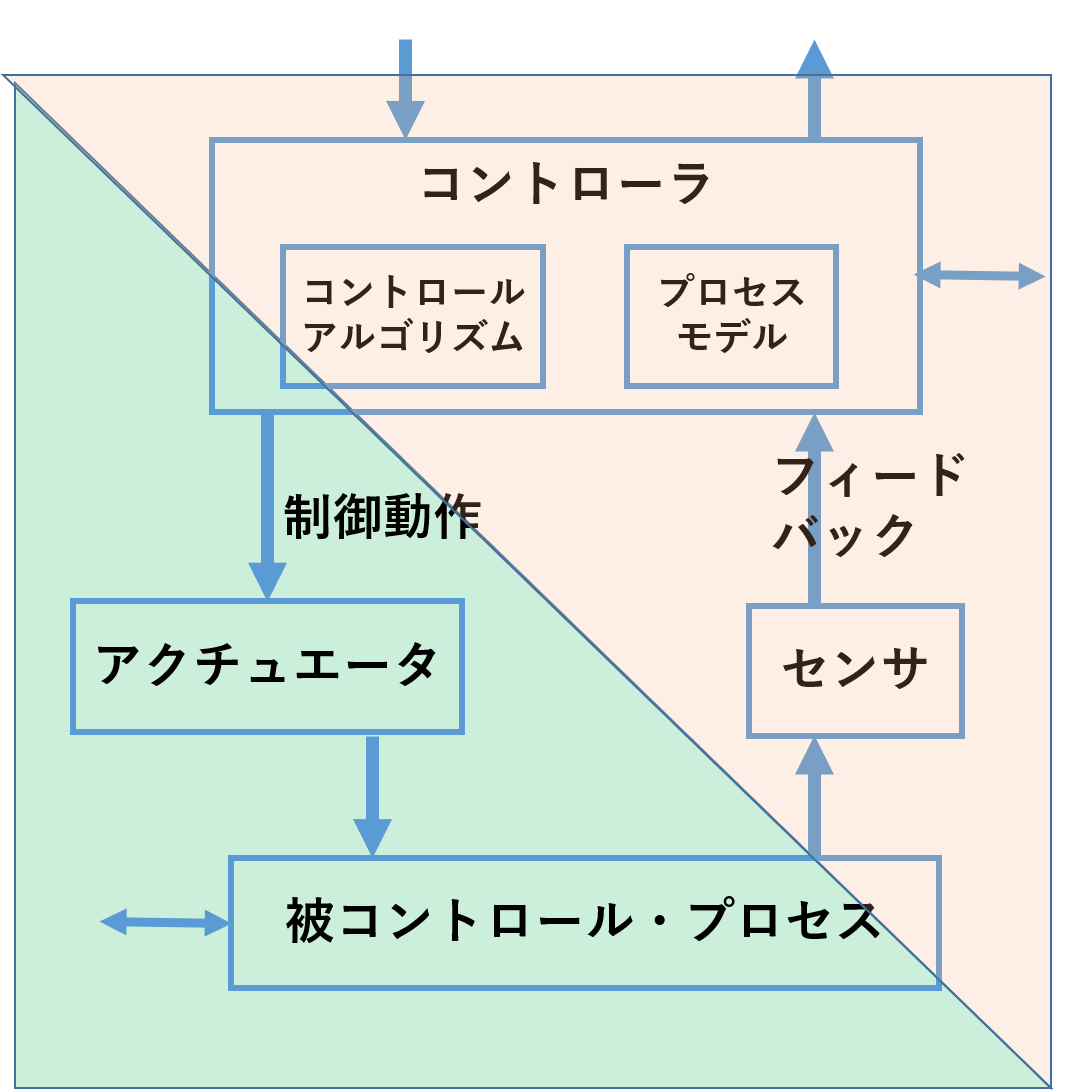
\includegraphics[width=40mm]{safety_assurance_contents/ch3images/fig-3-2-5-01.png}
    \caption[short]{考えるべきロスシナリオ}
\end{figure}

\textcolor{red}{(ハザードからロスシナリオまで一貫性・妥当性のある例に変更すること!)}
UCA「運転者からのブレーキ指示があり、タイヤがロックしていないにもかかわらず、ABSコントローラがブレーキ圧力発生を指示しないため,前方障害物との距離が規定値未満になる。」を考えます。
このUCAに対するロスシナリオ、特にUCAへ至るシナリオの例としては、
「センサからのフィードバックが間違っていたため、ABSコントローラがタイヤがロックしていないと誤認識してしまい、ABSコントローラがブレーキ圧力発生を指示しない。」が考えられます。
このように現実とプロセスモデル(コントローラの認識)が異なる状況は、プロセスモデルの不一致と呼ばれ、ロスシナリオを識別する際に、しばしば登場します。
また、制御動作の不実行・不適切な実行を表すシナリオの例としては、
「アクチュエータが故障していたため、ABSコントローラがブレーキ圧力発生を指示したにもかかわらず、アクチュエータがブレーキ圧力を発生しないため、自車両が減速せず障害物に衝突する。」が考えられます。



%%%%%%%%%%%%%%%%%%%%%%%%%%%%%%%%%%%%%%%%%%%%%%%%%%%%%%%%%%%%%%%%
\section{CAST(Causal Analysis based on System Theory)}
%%%%%%%%%%%%%%%%%%%%%%%%%%%%%%%%%%%%%%%%%%%%%%%%%%%%%%%%%%%%%%%%

CASTは、STAMPに基づく事故分析手法です。実際に発生したアクシデントのシナリオを識別し、システムの安全制御構造がなぜ機能しなかったかを分析します。

%%%%%%%%%%%%%%%%%%%%%%%%%%%%%%%%%%%%%%%%%%%%%%%%%%%%%%%%%%%%%%%%
\subsection{CASTの目的}

CASTの主な目的は以下の通りです:

\begin{itemize}
    \item 事故調査の際に問われるべき質問を特定する
    \item 事故がなぜ起こったのかを明らかにする
    \item 責任の所在を明らかにするのではなく、システムの改善点を見出す
\end{itemize}

%%%%%%%%%%%%%%%%%%%%%%%%%%%%%%%%%%%%%%%%%%%%%%%%%%%%%%%%%%%%%%%%
\subsection{CASTの手順}

CASTは以下の手順で実施されます:

\begin{enumerate}
    \item 基本情報の収集
    \item 安全コントロールストラクチャーのモデル化
    \item 損失における各コンポーネントの分析
    \item コントロールストラクチャーの欠陥の識別
    \item 改善プログラムの作成
\end{enumerate}

%%%%%%%%%%%%%%%%%%%%%%%%%%%%%%%%%%%%%%%%%%%%%%%%%%%%%%%%%%%%%%%%
\section{事例研究: 自動運転システムへのSTPAの適用}
%%%%%%%%%%%%%%%%%%%%%%%%%%%%%%%%%%%%%%%%%%%%%%%%%%%%%%%%%%%%%%%%

ここでは、自動運転システムにSTPAを適用する例を示します。

%%%%%%%%%%%%%%%%%%%%%%%%%%%%%%%%%%%%%%%%%%%%%%%%%%%%%%%%%%%%%%%%
\subsection{Step 1: 分析目的の定義}

\begin{itemize}
    \item ロス: 人命の損失、車両の損傷
    \item ハザード: 自車両と他の物体(車両、歩行者、障害物など)との距離が安全距離未満になる
    \item 安全制約: 自車両は常に他の物体との安全距離を維持しなければならない
\end{itemize}

%%%%%%%%%%%%%%%%%%%%%%%%%%%%%%%%%%%%%%%%%%%%%%%%%%%%%%%%%%%%%%%%
\subsection{Step 2: 制御構造図のモデル化}

% ここに制御構造図を挿入
\textcolor{red}{[自動運転システムの制御構造図を挿入]}

%%%%%%%%%%%%%%%%%%%%%%%%%%%%%%%%%%%%%%%%%%%%%%%%%%%%%%%%%%%%%%%%
\subsection{Step 3: 非安全制御動作の識別}

UCAの例:
\begin{itemize}
    \item UCA1: 前方に障害物があるにもかかわらず、自動運転システムがブレーキを適用しない
    \item UCA2: 安全な状況下で自動運転システムが不必要にブレーキを適用する
\end{itemize}

%%%%%%%%%%%%%%%%%%%%%%%%%%%%%%%%%%%%%%%%%%%%%%%%%%%%%%%%%%%%%%%%
\subsection{Step 4: ロスシナリオの識別}

ロスシナリオの例:
\begin{itemize}
    \item LS1: センサーの故障により、自動運転システムが前方の障害物を検知できず、ブレーキを適用しない
    \item LS2: ソフトウェアのバグにより、自動運転システムが安全な状況を危険と誤認識し、不必要にブレーキを適用する
\end{itemize}

%%%%%%%%%%%%%%%%%%%%%%%%%%%%%%%%%%%%%%%%%%%%%%%%%%%%%%%%%%%%%%%%
\section{事例研究: 鉄道システム事故へのCASTの適用}
%%%%%%%%%%%%%%%%%%%%%%%%%%%%%%%%%%%%%%%%%%%%%%%%%%%%%%%%%%%%%%%%

ここでは、実際の鉄道システム事故にCASTを適用する例を示します。

%%%%%%%%%%%%%%%%%%%%%%%%%%%%%%%%%%%%%%%%%%%%%%%%%%%%%%%%%%%%%%%%
\subsection{事故概要}

2019年6月1日、横浜シーサイドラインの無人自動運転列車が逆走し、終端の車止めに衝突した事故を分析します。

%%%%%%%%%%%%%%%%%%%%%%%%%%%%%%%%%%%%%%%%%%%%%%%%%%%%%%%%%%%%%%%%
\subsection{基本情報の収集}

\begin{itemize}
    \item 事故日時: 2019年6月1日 20時15分頃
    \item 場所: 新杉田駅
    \item 結果: 乗客25名中17名が負傷
    \item システム: 自動列車運転システム(ATO)、自動列車制御システム(ATC)
\end{itemize}

%%%%%%%%%%%%%%%%%%%%%%%%%%%%%%%%%%%%%%%%%%%%%%%%%%%%%%%%%%%%%%%%
\subsection{安全コントロールストラクチャーのモデル化}

% ここに安全コントロールストラクチャーの図を挿入
\textcolor{red}{[鉄道システムの安全コントロールストラクチャー図を挿入]}

%%%%%%%%%%%%%%%%%%%%%%%%%%%%%%%%%%%%%%%%%%%%%%%%%%%%%%%%%%%%%%%%
\subsection{各コンポーネントの分析}

例: ATOシステムの分析
\begin{itemize}
    \item 責任: 列車の自動運転制御
    \item 不適切な制御行動: 逆方向への出発指示
    \item 誤ったプロセスモデル: 正しい進行方向の認識の欠如
    \item コンテキスト: システムの設計上の欠陥
\end{itemize}

%%%%%%%%%%%%%%%%%%%%%%%%%%%%%%%%%%%%%%%%%%%%%%%%%%%%%%%%%%%%%%%%
\subsection{改善提案}

\begin{itemize}
    \item ATOシステムの進行方向認識機能の強化
    \item ATCシステムによる逆走検知機能の改善
    \item 人間のオペレーターによるバックアップ体制の強化
\end{itemize}

%%%%%%%%%%%%%%%%%%%%%%%%%%%%%%%%%%%%%%%%%%%%%%%%%%%%%%%%%%%%%%%%
\section{まとめ}
%%%%%%%%%%%%%%%%%%%%%%%%%%%%%%%%%%%%%%%%%%%%%%%%%%%%%%%%%%%%%%%%

STAMP/STPA及びCASTは、現代の複雑なシステムの安全性分析に適した手法です。これらの手法を用いることで、以下のような利点が得られます:

\begin{itemize}
    \item システム全体の安全性を包括的に分析できる
    \item 人間要因を含むシステムの相互作用を考慮できる
    \item 事故の根本原因だけでなく、システムの改善点を特定できる
    \item 設計段階から運用段階まで、システムのライフサイクル全体にわたって適用できる
\end{itemize}

これらの手法を効果的に活用することで、より安全で信頼性の高いシステムの開発と運用が可能になります。

%%%%%%%%%%%%%%%%%%%%%%%%%%%%%%%%%%%%%%%%%%%%%%%%%%%%%%%%%%%%%%%%
\section{参考文献}
%%%%%%%%%%%%%%%%%%%%%%%%%%%%%%%%%%%%%%%%%%%%%%%%%%%%%%%%%%%%%%%%
\begin{itemize}
    \item Engineering a Safer World, 2012
    \item STPA Handbook, 2018
    \item はじめてのSTAMP/STPA, 2016
    \item はじめてのSTAMP/STPA(実践編), 2017
    \item はじめてのSTAMP/STPA(活用編), 2018
    \item STAMPガイドブック ~システム思考による安全分析~, 2019
    \item STAMP Workbench
\end{itemize}
\chapter{モデルベースシステムズエンジニアリング}
%高井さん
\label{chap4}

\section{システムエンジニアリングの基礎}

\subsection{システムエンジニアリングとは}

システムエンジニアリングは、INCOSE SE HANDBOOKによると、「システムの実現を成功させることができる複数の専門分野にまたがるアプローチおよび手段」と定義されています。この分野は以下の役割を果たします:

\begin{itemize}
    \item システム開発に必要な概念の提供
    \item システム開発で必要な活動の提供
\end{itemize}

システムエンジニアリングは、分野に依存せず「システム」を構築したり発展
させたりするための知見をまとめたものです。従来は、製品やサービスの領域
毎に、開発プロセスは発展し、その中での最適化が行われてきました。しかし、
多くのシステムが大規模化、複雑化するなかで、領域毎に発展してきた方法論
では、必要な納期を満たせなかったり品質を保証することが難しくなってきま
した。一方で、そのような課題は、製品やサービスに依存しない現象として説
明したり、さらにはその解決アプローチについても、一般化して検討できるか
もしれない、と気付いた人たちがいました。そのような知見をまとめたものが
システムズエンジニアリングであり、実際多くの現場でその効果が確かめられ
たため、国際標準化なども含めて普及が進んでいます。

前述の通り、システムが大規模化、複雑化すると、複数の製品やサービス領域
を組み合わせることが一般的になり、これまで交流のなかった技術者も共同作
業をしなければなりません。そのようなときに共通言語を与えるのも、システ
ムズエンジニアリングの役割です。また、大規模かつ複雑なシステムは、その
開発や運用プロセスも複雑になり、その計画を立てたり、人員を割り当てる際
にも活動に関する共通言語が必要になります。それら開発や運用に係わる活動
に関する概念も、提供する共通概念の重要な部分です。

\subsection{システムエンジニアリングの知見}

システムエンジニアリングにはさまざまな知見が含まれますが、ここでは次の三つを紹介します:

\begin{enumerate}
    \item システムに関する概念の定義
    \item システムの開発や運用においてありうる活動の定義
    \item システムを記述するために必要な観点の提供
\end{enumerate}

\subsection{システムに関する概念の定義}

例えば、ジェットエンジンを開発するときには、巨大な試験施設が必要になり
ます。そのような施設もシステムであり、それ自体がライフサイクルを持ち、
試験対象であるジェットエンジンのライフサイクルも意識しながら施設を開発
し、運用する必要があります。開発や運用対象のシステムを対象システム
(system-of-interest)と呼ぶのに対し、開発時に連携が必要となるシステム
をイネーブリングシステム(enabling system)と呼びます
(図~\ref{figure:ch4-1})。
\begin{figure}
    \begin{center}
    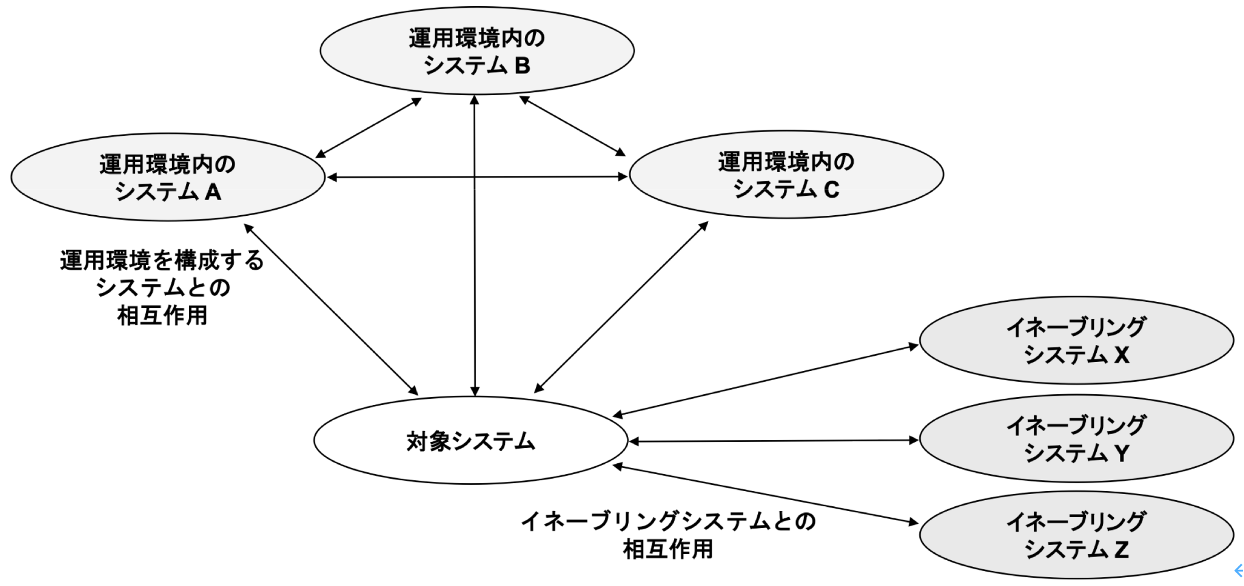
\includegraphics[width=100mm,bb=0 0 622 293]{safety_assurance_contents/ch4images/fig1.png}
    \caption{イネーブリングシステム}
    \label{figure:ch4-1}
    \end{center}
\end{figure}

\subsection{システムの開発や運用においてありうる活動の定義}

システムエンジニアリングでは、システム開発に関わる活動を分類し、標準化
したものとしてシステムライフサイクルプロセス(system lifecycle
  processes)が定義されています。ISO/IEC/IEEE 15288:2023による定義を
図~\ref{figure:ch4-2}に示します。
\begin{figure}
    \begin{center}
    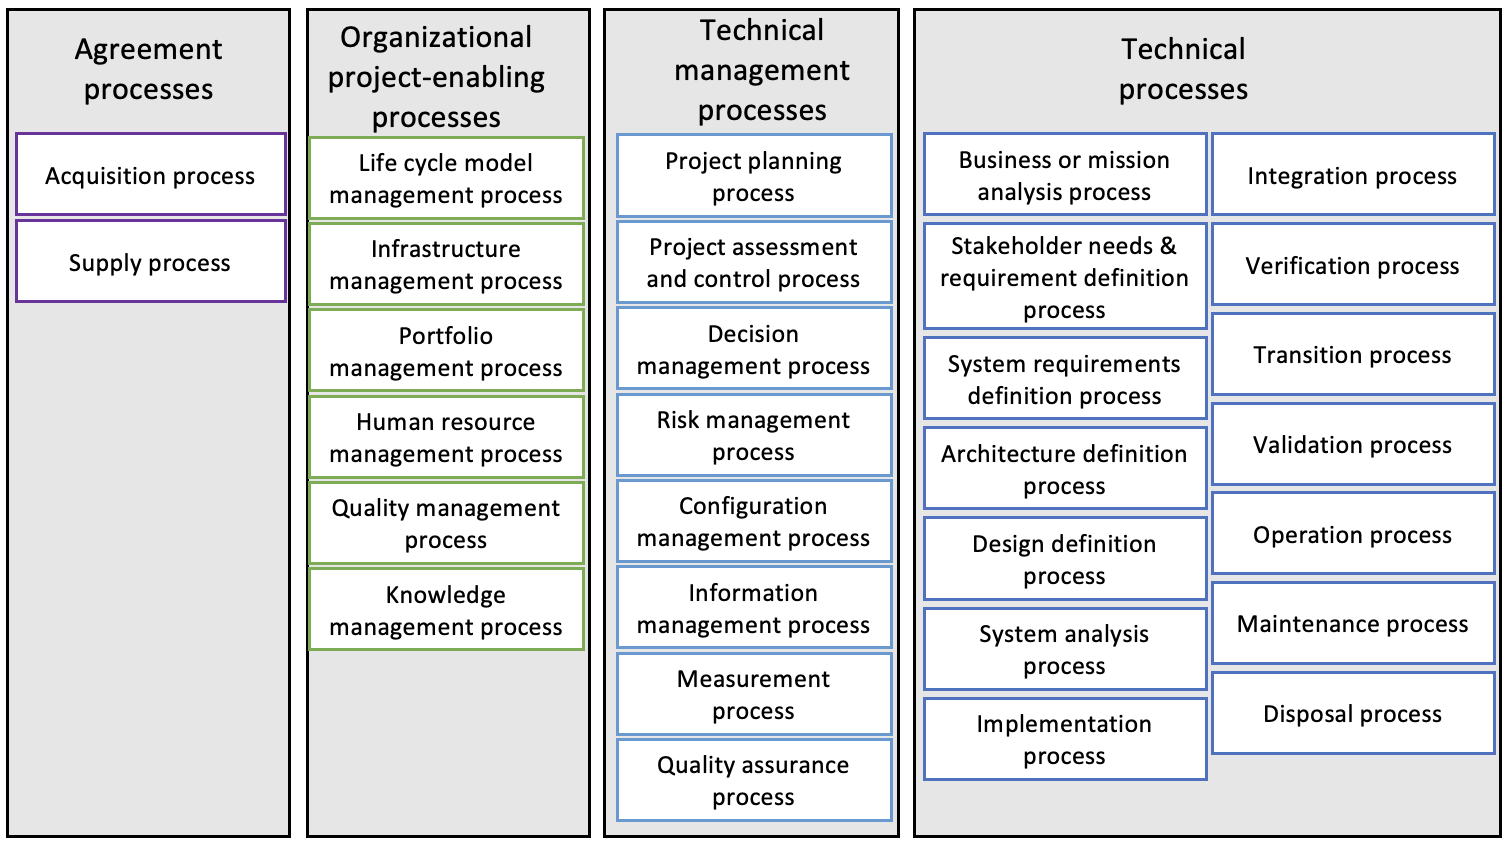
\includegraphics[width=100mm,bb=0 0 756 424]{safety_assurance_contents/ch4images/fig2.png}
    \caption{システムライフサイクルプロセス}
    \label{figure:ch4-2}
    \end{center}
\end{figure}

システムのライフサイクルに現れる活動は、ここに挙げられているどれかのプ
ロセスに相当すると考えることができます。注意点としては、これらのプロセ
スは順序を定義しているものではないということです。プロセスの順序は、ラ
イフサイクルモデル(lifecycle model)として定義され、異なる概念として
理解されます。

これらのライフサイクルプロセスは以下の4つに分類されます:

\begin{itemize}
    \item 合意プロセス(agreement processes)
    \item 組織のプロジェクトイネーブリングプロセス(organizational project-enabling processes)
    \item テクニカルマネジメントプロセス(technical management processes)
    \item テクニカルプロセス群(technical processes)
\end{itemize}

これらのプロセス群は、システムの直接的な開発活動だけでなく、それを支援
する活動も含んでいます。例えば、テクニカルプロセスには、技術者には馴染
み深い設計定義プロセス(design process)や実装プロセス
(implementation)、運用プロセス(operational process)などが含まれて
おり、イメージしやすいと思われます。一方で、システムズエンジニアリング
で提供されるライフサイクルプロセスはそれらだけではありません。プロジェ
クトを計画するプロジェクト計画プロセス(project planning process)や、
人員の確保や配置などの活動を含む人的リソースマネジメントプロセス
(human resource management process)、さらには、契約に係わる活動であ
る取得プロセス(acquisition process)や供給プロセス(supply process)
などまで含まれています。これは、これまでのシステムズエンジニアリングの
知見において、システムを開発する際には、直接的な開発活動だけでなく、そ
れを支える活動も含めて考える必要があることを表しています。

\subsection{システムを記述するために必要な観点の提供}

システムを開発したり、運用したりするためには、対象システムを記述する必
要があります。その記述方法についてもシステムズエンジニアリングは知見を
与えてくれます。

一般に、大規模なシステムは、一つの設計図だけではその全貌を現すことはで
きません。そのため、例えば、詳細な記述の前に、その概要だけを記した文章
や設計図なども作成します。従来からそのような記述を「アーキテクチャ設計」
や概要設計と呼んでいました。ただし、概要を把握するにしても、目的やそれ
を読む関係者に応じて複数の記述を作成することが一般的です。それではどの
ような記述が「アーキテクチャ」とよべるのでしょうか。アーキテクチャの記
述は一般にはシステムの抽象的なものです。ただし、抽象的であればアーキテ
クチャというわけでもありません。なぜ抽象化された記述なのに、それが利用
されるかと言えば、システムに関する何らかの関心事を表していたり、懸念事
項を確認できたりすることが期待されるからです。また、ここでの「関心事」
や「懸念事項」は、それを持つ主体が想定されます。システムに関して関心や
懸念を持つ主体を広くステークホルダー(stakeholder, 利害関係者)と呼び
ます。ここで、なんらかのしステークホルダーのなんらかの関心事(concern)
を表現したものをアーキテクチャビュー(architecture view)と呼びます。
アーキテクチャ記述(architecture description)は、このビューの集まりで
あると定義されます。

さらに、ステークホルダーとその関心事は、典型的なものはパターン化してお
くと便利であり、かつ、その記述方法は、おのずと適切に表現できる記法がき
まってくることが多いです。このような、ステークホルダーとその関心事、そ
の表現方法をまとめたものをアーキテクチャビューポイント(architecture
  viewpoint)と呼ばれます。アーキテクチャビューとアーキテクチャビュー
ポイントのイメージは次のような図で説明されることがありま
す~(\ref{figure:ch4-3})。

\begin{figure}
    \begin{center}
    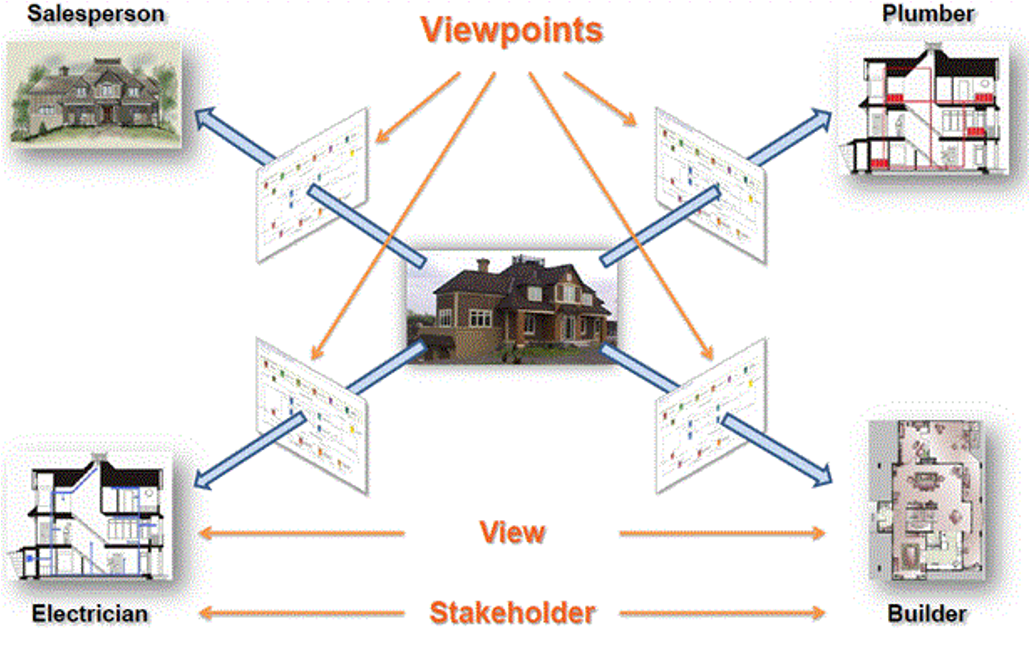
\includegraphics[width=100mm,bb=0 0 515 323]{safety_assurance_contents/ch4images/fig3.png}
    \caption{アーキテクチャビュー及びアーキテクチャビューポイントのイメージ}
    \label{figure:ch4-3}
    \end{center}
\end{figure}

原理的にはシステム毎にステークホルダーやその関心事は異なるため、アーキ
テクチャビューポイントはシステム開発のプロジェクト毎に構築しなければな
らないように見えますが、一般的に多くのプロジェクトで使用可能なアーキテ
クチャビューポイントの集まりもいくつか提供されています。ここでは、その
中からアーキテクチャビューポイントの具体例を紹介します。

\begin{itemize}
\item オペレーショナルビューポイント
  \begin{itemize}
\item ステークホルダー $\colon$ ビジネスアーキテクト、経営層
\item 関心事 $\colon$ 対象の論理的なアーキテクチャを明らかにする。
  \end{itemize}
\end{itemize}
ここで提供されている「オペレーショナルビューポイント」のステークホルダー
は、経営層やビジネスアーキテクトと呼ばれる人たちです。関心事の「論理的
  なアーキテクチャ」とは、実現方法や実装方法に依存しない論理的な構造や
振る舞いを記述するアーキテクチャを指します。もし対象システムのステーク
ホルダーに経営層やビジネスアーキテクト相当の人たちが係わっている場合、
まずはこのような一般的に提供されているビューポイントから、それらステー
クホルダーに関係しそうなビューポイントの記述を参考に、必要なビューポイ
ントを定義することができます。

\section{モデルベースドシステムズエンジニアリング(MBSE)}

\subsection{MBSEの概念}

モデルベースドシステムズエンジニアリング(model-based systems
  engineering, MBSE)は、モデルを活用したシステムエンジニアリングのア
プローチです。ここでいうモデルとは、ある対象に対して、その対象の特徴を
理解したり予測したりするために用いられる抽象的な表現を指します。

\subsection{SysML(Systems Modeling Language)}

SysMLは、システムエンジニアリングのための代表的なモデリング言語です。
UML(Unified Modeling Language)をベースに定義されており、システムを以
下の四つの側面から記述することが可能です:

\begin{enumerate}
    \item 構造
    \item 振る舞い
    \item パラメータ間の関係
    \item 要求
\end{enumerate}

\section{SysMLを用いたシステムモデリング}

\subsection{構造のモデリング}

構造のモデリングでは、システムを構成する要素とその関係を表現します。例
えば、自動車システムの場合、エンジン、シャーシ、車体などの構成要素とそ
れらの関係を表現します。

\subsection{振る舞いのモデリング}

振る舞いのモデリングでは、システムの動作や状態遷移を表現します。例えば、
自動車の運転プロセスや、エンジンの始動から停止までの状態遷移などを表現
します。

\subsection{パラメータ間の関係のモデリング}

パラメータ間の関係のモデリングでは、システムの性能や特性を決定する要因
間の関係を表現します。例えば、自動車の場合、エンジン出力と最高速度の関
係、車体重量と燃費の関係などを表現します。

\subsection{要求のモデリング}

要求のモデリングでは、システムが満たすべき条件や制約を表現します。例え
ば、自動車の場合、安全性基準、燃費基準、排出ガス規制などの要求を表現し
ます。

\section{トレードオフ分析}

\subsection{トレードオフ分析の概要}

トレードオフ分析は、システムの異なる特性や性能間の関係を評価し、最適な解決策を見出すプロセスです。多くの場合、ある特性を向上させると他の特性が低下するという関係があり、これらのバランスを取ることが重要です。

\subsection{記述型モデルと分析型モデルの連携}

トレードオフ分析を効果的に行うためには、記述型モデルと分析型モデルの連携が重要です。

\begin{itemize}
    \item 記述型モデル:SysMLなどを用いて、システムの構造、振る舞い、要求などを記述します。ステークホルダー間のコミュニケーションや合意形成に役立ちます。
    \item 分析型モデル:MATLAB/Simulinkなどのツールを用いて、システムの性能や動作をシミュレーションします。定量的な評価や予測に役立ちます。
\end{itemize}

\subsection{トレードオフ分析の手順}

以下の手順でトレードオフ分析を行います:

\begin{enumerate}
    \item ソリューション案の検討と妥当性確認
    \item 分析ケースの検討と妥当性確認
    \item パラメータ項目/値の検討と妥当性確認
    \item シミュレーションなどによる分析の実施
    \item 分析結果の評価と意思決定
\end{enumerate}

\section{事例研究: 自動駐車システム}

ここでは、自動駐車システムの設計と評価を例に、システムエンジニアリングの実践を見ていきます。

\subsection{システム概要}

想定する自動駐車システムは以下の特徴を持ちます:

\begin{itemize}
    \item ショッピングセンター近くの巨大な立体駐車場を対象
    \item 利用者は駐車場入口でクルマから降り、アプリで自動駐車を指示
    \item 車両は自律的に空きスペースまで移動し駐車
    \item 引き取り時も、アプリで指示後に車両が自動で出庫
\end{itemize}

\subsection{能力の定義と評価指標}

システムに求められる能力とその評価指標を定義します:

\begin{itemize}
    \item 能力:自動駐車機能
    \item 評価指標:
    \begin{itemize}
        \item 平均入庫時間
        \item 平均出庫時間
        \item 平均待ち時間
        \item 安全度レベル
        \item 利用者ストレスポイント
    \end{itemize}
\end{itemize}

\subsection{リソースアーキテクチャの検討}

システムを構成するリソースとその構造を検討します。主要なコンポーネントには以下が含まれます:

\begin{itemize}
    \item 自動運転機能付き車両
    \item 駐車場管理システム
    \item 空きスペース確認システム(固定カメラまたはドローン)
    \item ユーザーインターフェース(スマートフォンアプリ)
\end{itemize}

\subsection{分析ケースの定義}

システムの評価のための分析ケースを定義します。考慮すべき要素には以下が含まれます:

\begin{itemize}
    \item 自動運転車普及率(例:20%、80%)
    \item 来客状況(閑散期、繁忙期)
    \item 駐車場の構造と容量
    \item 周辺交通状況
\end{itemize}

\subsection{シミュレーションと分析}

定義した分析ケースに基づき、MATLAB/Simulinkなどのツールを用いてシミュレーションを行います。また、STAMP/STPAなどの手法を用いて安全性分析を実施します。

\subsection{結果の評価とトレードオフ分析}

シミュレーションと分析の結果を評価し、各ソリューション案のトレードオフを検討します。例えば:

\begin{itemize}
    \item 固定カメラ方式:初期コストは低いが、スケーラビリティに課題
    \item ドローン方式:柔軟性が高いが、安全管理に追加コストが必要
\end{itemize}

これらの結果を総合的に判断し、最適なソリューションを選択します。

\section{まとめ}

システムエンジニアリングは、複雑なシステムの開発と管理を体系的に行うための重要なアプローチです。MBSEやSysMLの活用、そしてトレードオフ分析の実施により、以下のような利点が得られます:

\begin{itemize}
    \item システムの全体像と詳細の両方を把握できる
    \item ステークホルダー間のコミュニケーションが促進される
    \item 定量的な評価に基づく意思決定が可能になる
    \item システムの品質、信頼性、安全性の向上につながる
\end{itemize}

今後のシステム開発者は、これらの手法と考え方を効果的に活用し、より良いシステムを設計・開発することが求められます。


\chapter{アシュアランスケースとGSN}
\label{chap5}



\section{アシュアランスケースとは}

アシュアランスケース(Assurance Cases)は、システムまたは製品の特性(安全性、セキュリティ、信頼性など)に関して、構造化された議論を明示的に示すドキュメントです。このドキュメントは、最上位の主張を下位の証拠および前提条件に結びつける形で構成されます。

特に安全性に焦点を当てたアシュアランスケースは、セーフティケース(Safety Case)と呼ばれます。セーフティケースは、機能安全や自動運転開発の分野で広く推奨されており、以下のような規格で言及されています:

\begin{itemize}
    \item ISO 26262(自動車の機能安全規格)
    \item SOTIF(ISO/PAS 21448, UL4600)
\end{itemize}

\section{MISRA Safety Case Guideline}

MISRA(Motor Industry Software Reliability Association)は、ISO 26262に準拠したSafety Caseを作成するためのガイドラインを提供しています。このガイドラインでは、安全性の議論を以下のような層構造で捉えています:

\begin{enumerate}
    \item Core(核心): 適切な要求事項を得たか
    \item Layer 1(第1層): 要求事項を満たしたか
    \item Layer 2(第2層): 適切な手段を用いたか
    \item Layer 3(第3層): 適切な環境で開発したか
\end{enumerate}

この構造に基づいて、自動車の安全性に関する議論は以下のように展開されます:

\begin{itemize}
    \item 自動車は完全で正しい安全ゴールの通りに動作する
    \item 自動車はハザードイベントiを低減する安全ゴールiの通りに動作する
    \item 安全ゴールiの妥当性
    \item 自動車の安全ゴールiへの準拠性
    \item 自動車の安全ゴールiの達成手段
    \item 自動車の安全ゴールiの開発手段
\end{itemize}



\section{セーフティケースの重要性}

セーフティケースの重要性は、過去の事例からも明らかです。例えば、2009年から2010年にかけて発生したトヨタ自動車のスロットル制御システムの問題では、安全性に関する明確な説明や証拠の提示が不足していました。この事例は、「それらを明確に用意できていれば、もっと簡単に解決していた(かもしれない)」という教訓を残しました。

このような経験から、システムの安全性や信頼性に関する説明責任の重要性が高まっています。アシュアランスケースは、この説明責任を果たすための効果的なツールとなります。

\section{D-Caseの概要と基本原則}

\subsection{D-Caseとは}

D-Caseは、JST CREST DEOSプロジェクトのD-Caseコアチームによって2009年から2013年にかけて開発された手法です。名称の「D」は「Dependability(信頼性)」を表しています。

D-Caseの主な目的は以下の通りです:

\begin{itemize}
    \item 合意形成のための手法・ツールの提供
    \item 開発・運用を通じたアシュアランスケースによるディペンダビリティの合意形成
\end{itemize}

\section{D-Caseの目的: ミニマムの合意形成}

D-Caseの核心的な目的は、異なる立場や背景を持つステークホルダー間での「ミニマムの合意形成」を実現することです。以下の図は、この概念を視覚的に表現しています:

% ここにD-Caseの合意形成の図を挿入する
\textcolor{red}{[D-Caseの合意形成の図を挿入]}

この図が示すように、D-Caseは以下のプロセスを促進します:

\begin{enumerate}
    \item 異なる立場・関心・目的、経験・価値観を持つステークホルダーを特定する
    \item それぞれのステークホルダーの前提・主張を明確にする
    \item 共通の目的・前提を設定し、合意形成を図る
\end{enumerate}

\subsection{D-Caseの基本的な考え方}

D-Caseを効果的に活用するための基本的な考え方は以下の通りです:

\begin{itemize}
    \item GSN(Goal Structuring Notation)自体は基本的な構造にとどめ、大きすぎないようにする
    \item コンテキストには要求分析結果、安全分析結果、テスト結果などの詳細なドキュメントを配置する
    \item GSN自体は様々なドキュメントを紐付ける論理的な骨組みとして機能させる
    \item 他のドキュメントが充実していれば、GSN自体は迅速に作成できるようにする
\end{itemize}

この考え方により、D-Caseは複雑なシステムの信頼性を効率的に議論し、合意形成を促進するツールとなります。

\section{GSN(Goal Structuring Notation)}

\subsection{GSNの概要}

GSN(Goal Structuring Notation)は、アシュアランスケースを視覚的に表現するためのグラフィカル記法です。GSNは以下のような特徴を持ちます:

\begin{itemize}
    \item 議論のモデル化を可能にする
    \item 様々な目的で利用できる柔軟性がある
    \item 元々はシステムの安全性を保証するためのセーフティケースを記述する目的で開発された
    \item D-Caseにおいて中心的な役割を果たす
\end{itemize}

\section{GSNの基本要素}

GSNは以下の基本的なノードを使用して構成されます:

\begin{description}
    \item[ゴール(Goal)] ステークホルダ間で合意したい主張
    \item[戦略(Strategy)] 上位のゴールの分解の仕方を説明
    \item[前提(Context)] 議論の前提となる情報
    \item[証拠(Evidence)] ゴールが達成できていることを示す証拠(テスト結果など)
    \item[未達成(Undeveloped)] まだ具体化できていないゴールや説明であることを示す
\end{description}

% ここにGSNの基本要素の図を挿入する
\textcolor{red}{[GSNの基本要素の図を挿入]}

\subsection{GSNのノード接続ルール}

GSNのノードを接続する際は、以下のルールに従います:

\begin{itemize}
    \item 「前提」に接続する場合はコンテキストリンク(点線)を使用
    \item それ以外の接続にはサポートリンク(実線)を使用
    \item 終端は必ず「証拠」か「未達成」
    \item 「ゴール」は「戦略」に基づきサブゴールに分解する
\end{itemize}

% ここにGSNのノード接続ルールの図を挿入する
\textcolor{red}{[GSNのノード接続ルールの図を挿入]}

\subsection{GSNの作成例}

以下に、GSNの簡単な作成例を示します。この例では、システムの安全性を主張するためのGSNを構築しています。

% ここにGSNの簡単な例の図を挿入する
\textcolor{red}{[GSNの簡単な例の図を挿入]}

この例では、以下の要素が含まれています:

\begin{itemize}
    \item トップゴール:「システムは安全である」
    \item 戦略:「ハザードごとに議論する」
    \item サブゴール:「ハザードAに対処できる」「ハザードBに対処できる」
    \item 前提:「ハザードリストA,B」
    \item 証拠:「テスト結果」
\end{itemize}

このように、GSNを用いることで、システムの安全性に関する議論を構造化し、視覚的に表現することができます。

\section{D-Caseステップ}

\subsection{D-Caseステップの概要}

D-Caseステップは、システム開発や日常の場で異なるステークホルダが手軽に合意形成を行うためのプロセスです。このプロセスは、システム開発における様々なミスコミュニケーションを減らし、ディペンダビリティを向上させることを目的としています。

D-Caseステップは以下の3つのステップから構成されます:

\begin{enumerate}
    \item ステークホルダの設定
    \item D-Caseの記述
    \item 合意形成の実施
\end{enumerate}

\subsection{ステップ1:ステークホルダの設定}

このステップでは、プロジェクトや議論に関わる全てのステークホルダを特定します。ステークホルダには、開発者、利用者、運用者など、システムに関わる全ての人々が含まれます。

ステークホルダを明確化することで、以下の利点があります:

\begin{itemize}
    \item 各ステークホルダの立場・関心・考え・経験・価値観を理解できる
    \item ステークホルダ間の潜在的な対立や誤解を事前に特定できる
    \item 合意形成のプロセスをスムーズに進められる
\end{itemize}

\subsection{ステップ2:D-Caseの記述}

D-Caseの記述は、以下の3段階で行います:

\begin{enumerate}
    \item 「前提」とトップの「ゴール」を設定する
    \item 「戦略」を設定し、トップゴールを分割してサブの「ゴール」を設定する
    \item それぞれの最終ゴールのための「証拠」(または「未達成」)を設定する
\end{enumerate}

この過程で、以下の点に注意します:

\begin{itemize}
    \item これまでのD-Caseがあれば参照する
    \item 設定したステークホルダの情報を考慮する
    \item 論理的な構造を保ちながら、詳細化していく
\end{itemize}

\subsection{ステップ3:合意形成の実施}

合意形成の実施には、以下の2つの場合があります:

\begin{description}
    \item[ステークホルダ全員の場合] プロジェクタ等でD-Caseを表示しながら、合意ができるか議論する
    \item[一部のステークホルダのみの場合] D-Case記述不参加のステークホルダにもわかるよう合意形成を行う。必要であればD-Caseと同等の情報量を持つ絵や文章を用意する
\end{description}

\subsection{D-Caseの評価基準}

作成したD-Caseは、以下の3つの観点から評価します:

\begin{description}
    \item[前提の妥当性] 前提が過不足なく配置されているか
    \item[議論の妥当性] 議論が論理的でステークホルダが理解できるか
    \item[規模の妥当性] ステークホルダが理解できる規模か
\end{description}

評価の結果、改善が必要な場合は、これらの基準に基づいてD-Caseを修正します。一般的に、スライド1枚で見えるくらいの規模が目安となります。

\section{事例紹介:自動運転システム}

\subsection{レベル4自動運転システムの事例}

ここでは、レベル4自動運転システムを継続的に保証するための枠組みを提案した事例を紹介します。この事例は、SafeComp 2024で発表された「A Case Study of Continuous Assurance Argument for Level 4 Automatic Driving」に基づいています。

主な特徴:

\begin{itemize}
    \item\item 塩尻駅から塩尻市庁舎の周回コース(2km)を対象とする
    \item 特に市役所へ入るための右折にフォーカス
    \item STAMP/STPAの分析結果などをもとにGSNを記述
\end{itemize}

この事例研究では、自動運転シャトルバスが直面する様々な信頼性の課題に焦点を当てています。例えば、道路上の物体に対する過度に保守的な安全マージンは、車両が無期限に右折できなくなる可能性があり、交通システム全体の可用性を低下させる可能性があります。

\subsection{継続的アシュアランスの重要性}

この研究では、静的なアシュアランスケースだけでなく、継続的なモニタリングデータを組み合わせた動的なアプローチの重要性を強調しています。UL4600(自動運転車の国際標準)で導入されている安全性能指標(SPIs)は、この考え方を反映したものです。

SPIsは、設計、シミュレーション、テスト、展開の各段階で安全性主張が反証されていないかを検出する手段を提供します。著者らが提案するモニタリングシステムを含むツールチェーンは、このSPIメカニズムの一例と言えます。

\subsection{アシュアランスケースのトップレベル構造}

レベル4自動運転システムのアシュアランスケースのトップレベル構造は、以下のような要素で構成されています:

\begin{itemize}
    \item システムの安全性に関する最上位の主張
    \item 運用条件、環境条件などの前提
    \item サブシステムごとの安全性主張
    \item 妥当性検証と評価に関する主張
\end{itemize}

% ここにアシュアランスケースのトップレベル構造の図を挿入する
\textcolor{red}{[アシュアランスケースのトップレベル構造の図を挿入]}

\subsection{特定のユースケースの妥当性検証}

この事例研究では、塩尻市での特定のユースケース(市役所への右折)に焦点を当てた妥当性検証のGSN図も提示されています。この図は、以下のような要素を含んでいます:

\begin{itemize}
    \item ユースケースの安全性に関する主張
    \item 安全性要求事項の充足性
    \item テストシナリオの網羅性
    \item 実環境でのテスト結果
\end{itemize}

% ここに特定のユースケースの妥当性検証のGSN図を挿入する
\textcolor{red}{[特定のユースケースの妥当性検証のGSN図を挿入]}

この詳細なGSN図は、特定のユースケースに対する安全性の議論を構造化し、必要な証拠と論理的つながりを明確に示しています。

\section{まとめ}

本書では、システムのディペンダビリティを確保するための重要なツールであるアシュアランスケースとGSNについて学びました。主な内容は以下の通りです:

\begin{itemize}
    \item アシュアランスケース:システムが信頼できることを示すドキュメント
    \item GSN(Goal Structuring Notation):グラフィカルなアシュアランスケースの表記法、モデル
    \item D-Case:ステークホルダ間の合意形成を促進するための手法
    \item 自動運転システムなどの最近のシステムでの実践例
\end{itemize}

これらの手法と概念は、今日の複雑化するシステム開発において、信頼性、安全性、セキュリティを確保するために不可欠なものとなっています。特に、自動運転技術やAIシステムなど、新しい技術の導入に伴い、システムの振る舞いの予測が困難になる中で、アシュアランスケースの重要性はますます高まっています。

今後のシステム開発者は、これらの手法を効果的に活用し、システムの信頼性を体系的に示す能力を磨くことが求められます。同時に、継続的なモニタリングと評価を通じて、システムの安全性と信頼性を維持・向上させていく必要があります。

アシュアランスケースとGSNは、単なる文書化ツールではなく、システム開発のプロセス全体を通じて、安全性と信頼性に関する思考を構造化し、ステークホルダ間のコミュニケーションを促進する強力な手段です。これらを適切に活用することで、より安全で信頼性の高いシステムの開発が可能となるでしょう。

\section{D-Caseの実践演習:スマート内覧システム}

本節では、D-Case手法を用いた合意形成の可視化を体験し、D-Caseステップを実践的に学ぶための演習を行います。

\subsection{演習の概要}

\subsubsection{演習の目的}
\begin{itemize}
    \item D-Case手法による合意形成の可視化を体験する
    \item D-Caseステップを実践的に確認する
\end{itemize}

\subsubsection{演習の流れ}
\begin{enumerate}
    \item テーマ説明
    \item ステークホルダの設定
    \item D-Caseの記述
    \item 合意の実施
\end{enumerate}

\subsection{テーマ:スマート内覧システム}

本演習では、「スマート内覧」というサービスを題材とします。これは、ユーザーの携帯電話を利用してセルフ(ひとり)で不動産物件の内覧ができるサービスです。

\subsubsection{スマート内覧システムの特徴}
\begin{itemize}
    \item 事前予約による無人内覧
    \item ユーザー認証による鍵のロック解除
    \item 専用タブレットによる案内
    \item 制限時間内は自由に見学可能
    \item 終了5分前にタブレットによる通知
    \item カメラ越しの監視付き(事前連絡あり)
    \item 終了後、ユーザーが施錠を確認
\end{itemize}

\subsection{ステップ1:ステークホルダ分析}

\subsubsection{ステークホルダの特定}
このシステムに関わる全てのステークホルダを特定します。例えば:
\begin{itemize}
    \item 開発会社
    \item 管理会社
    \item ユーザー(物件内覧者)
    \item 不動産所有者
    \item 地域住民
\end{itemize}

\subsubsection{ステークホルダ関係の設定}
どのステークホルダ間の関係性についてD-Caseを描くかを決定します。例:
\begin{itemize}
    \item 開発会社 から ユーザー
    \item 管理会社 から 開発会社
    \item 開発会社 から 管理会社
\end{itemize}

\textbf{注意点:} どういったステークホルダが存在するかを明確にし、ステークホルダ間の説明責任を分析することが重要です。

\subsection{ステップ2:D-Caseの記述}

\subsubsection{「前提」の抽出}
選択したステークホルダ関係に基づいて、以下の項目を抽出します:
\begin{itemize}
    \item 要求(2つ以上)
    \item 懸念事項(2つ以上)
\end{itemize}

例:
\begin{description}
    \item[要求:] 
    \begin{itemize}
        \item システムは安全に動作する
        \item 誤動作が少ない
    \end{itemize}
    \item[懸念事項:] 
    \begin{itemize}
        \item システムに問題はないのか
        \item セキュリティ、動作の問題
    \end{itemize}
\end{description}

\textbf{注意点:} 「誰」から「誰」に対して「どのような」説明責任があるかを意識してください。

\subsubsection{「トップゴール」の設定}
要求や懸念事項に対して「何の」説明責任があるかを意識し、トップゴールを設定します。

例:「スマート内覧システムによって懸念される事項が起こらない」

\subsubsection{「前提」の設定}
トップゴールに対して関連する前提を接続します。これらの前提は、後の展開のガイドとなります。

例:
\begin{itemize}
    \item セキュリティー面(窓、鍵の施錠)
    \item ユーザーによる破損行為等
    \item システムが問題なく動作する
    \item 管理会社へのメリット
\end{itemize}

\subsubsection{「戦略」の決定}
トップゴールをどのようなサブゴールに分割するかという方針を「戦略」として記述します。

例:「懸念事項ごとに議論する」

他の戦略の例:
\begin{itemize}
    \item 安全性の10項目で議論する
    \item ユーザーの懸念事項と期待で分けて議論する
    \item サブシステムごとに安全性を議論する
    \item ハザードごとに議論する
\end{itemize}

\subsubsection{「サブゴール」の設定}
戦略に基づいて、トップゴールをサブゴールに細分化します。

例:
\begin{itemize}
    \item セキュリティー面(窓、鍵の施錠)の対策
    \item システムが問題なく動作する
    \item 管理会社へのメリットがある
    \item 破損行為等への対策がある
\end{itemize}

\subsubsection{「証拠」の設定}
各サブゴールに対して、それを達成したことを証明できる証拠を設定します。

例:「施錠は完璧にされる」というサブゴールに対して、「施錠実験結果」を証拠として設定。

\subsection{ステップ3:合意形成の実施}

\begin{itemize}
    \item 説明相手を想定し、作成したD-Caseを用いて合意を実施します。
    \item GSNを理解していない相手もいるため、必要に応じて別の表現方法も用意します。
    \item わかりやすく、伝わりやすい説明を心がけます。
\end{itemize}

\subsection{D-Caseの評価}

作成したD-Caseを以下の観点から評価します:

\begin{enumerate}
    \item 前提の妥当性:前提が過不足なく配置されているか
    \item 議論の妥当性:議論が論理的でステークホルダが理解できるか
    \item 規模の妥当性:ステークホルダが理解できる規模か
\end{enumerate}

\subsection{演習課題}

\begin{enumerate}
    \item スマート内覧システムについて、開発会社からユーザーへの説明責任を想定したD-Caseを作成してください。
    \item 作成したD-Caseについて、グループ内で相互評価を行い、改善点を議論してください。
    \item 改善したD-Caseを用いて、ユーザー役の人に対して説明を行い、フィードバックを得てください。
    \item 最終的なD-Caseと、演習を通じて学んだことをレポートにまとめてください。
\end{enumerate}

この演習を通じて、アシュアランスケースの実践的な作成方法と、ステークホルダ間のコミュニケーションにおけるその有用性を理解することができるでしょう。



\chapter{総合演習:自動運転システムの信頼性分析}
\label{chap6}

本章では、これまでに学んだ知識を活用し、STAMP/STPA(System-Theoretic Process Analysis)を用いて自動運転システムの信頼性分析を行います。この演習を通じて、実際のシステム開発における安全性分析の手法を体験的に学びます。

\section{演習の概要}

\subsection{対象システム}
自動運転車の事例:L4 自動車駐車誘導(L4 Car Park Pilot,L4 CPP)

\subsection{想定シナリオ}
自動運転車サービスを提供する会社を想定します。要求分析の結果、以下のような要求仕様が固まってきました:

\begin{itemize}
    \item なんらかの認証がなされた駐車場又は駐車エリア内において、無人での移動を行う。
    \item 最大速度は10km/h。
    \item 危険を検知したときのアクション:
    \begin{enumerate}
        \item 車速を徐行速度まで落とす。ただし、交差地点や合流箇所には進入しない。
        \item 安全地帯で停止し、(もしいれば)遠隔オペレーター、又は、ドライバーに通知する。
    \end{enumerate}
\end{itemize}

\subsection{目指す安全状態}
\begin{enumerate}
    \item 車両は徐行速度で運転され、衝突を回避している。
    \item 安全な場所で停止し、セキュアな状態にある。遠隔オペレーター又はドライバーは情報を通知され、今後の対処について決定している。
\end{enumerate}

\section{システム要素の概要}

本演習では、以下のようなシステム要素を考慮します:

\subsection{Localization(位置推定のためのセンシングシステム)}
駐車場内の駐車場所を特定するのに十分な精度を持つ。実装方法は、例えば、駐車場の地図情報と、人工的なランドマークを配置するなどの方法が考えられる。

\subsection{Environmental Perception Sensor(物標検知のためのセンシングシステム)}
前方などの障害物や他車両、歩行者、駐車場構造物、路上の標識やラインなどを検知する。必要に応じて駐車場との通信も可能。

\subsection{Interpretation and Prediction(解釈と予測システム)}
他車両や歩行者、その他障害物などの動きの意味を解釈し、未来の動きを予測する。

\subsection{Driving Planning(運転計画システム)}
走行経路を計画し、計画された走行経路に対し、走行路の条件や自車の幅、他の物標などの制限を考慮し、車両の縦方向及び横方向の運動に変換する。

\subsection{ADS Mode Manager(自動運転モード管理システム)}
自動運転モードの起動条件と解除条件をチェックする。縮退モードへの遷移も担う。

\subsection{User State Determination(ユーザー状態決定システム)}
ユーザー(任意の搭乗者)が運転機能の委譲を要求しているか検出する。

\subsection{Monitors(監視システム)}
長時間のオペレーションになる場合、電源又は燃料を監視する。

\section{STAMP/STPAによる安全分析の手順}

STAMP/STPAを用いた安全分析は、以下の手順で行います:

\begin{enumerate}
    \item 分析目的の定義
    \begin{itemize}
        \item ロス、アクシデント、ハザード、安全制約の識別
    \end{itemize}
    \item 制御構造図のモデル化
    \item 非安全制御動作(UCA: Unsafe Control Action)の識別
    \item ロスシナリオの識別
\end{enumerate}

\section{演習課題}

以下の手順に従って、L4 自動車駐車誘導システムの安全分析を行ってください。

\subsection{ロス(アクシデント)とハザードの識別}
システムが引き起こす可能性のあるロス(アクシデント)とハザードを特定してください。

\textbf{例:}
\begin{itemize}
    \item ロス:人身事故、車両損傷
    \item ハザード:他の車両や歩行者との衝突、駐車場構造物との接触
\end{itemize}

\subsection{制御構造図のモデル化}
システムの制御構造図を作成してください。各コンポーネント間の制御アクションと、フィードバック情報を明確に示してください。

\subsection{非安全制御動作(UCA)の識別}
各制御アクションに対して、以下の4つの類型に基づいてUCAを識別してください:

\begin{enumerate}
    \item 必要な制御アクションが与えられない
    \item unsafe な制御アクションが与えられる
    \item 制御アクションのタイミングまたは順序が適切でない(早すぎる、遅すぎる、正しくない順序)
    \item 制御アクションの継続時間が不適切(停止が早すぎる、適用され過ぎる)
\end{enumerate}

\textbf{UCA表の例:}
\begin{table}[h]
\caption{UCA表の例}
\begin{tabular}{|p{3cm}|p{3cm}|p{3cm}|p{3cm}|}
\hline
制御アクション & 与えない & 与える & タイミング/順序 \\
\hline
ブレーキ制御 & ブレーキを適用しない場合、衝突の危険がある & 不必要なブレーキにより後続車との衝突の危険がある & ブレーキが遅すぎると衝突の危険がある \\
\hline
\end{tabular}
\end{table}

\subsection{ロスシナリオの識別}
特定したUCAに対して、それがなぜ発生する可能性があるのかを分析し、ロスシナリオを作成してください。

\textbf{ロスシナリオの例:}
\begin{itemize}
    \item センサーの故障により障害物を検知できず、ブレーキが適用されない。
    \item ソフトウェアのバグにより、不適切なタイミングでブレーキが適用される。
\end{itemize}

\section{レポート作成}

演習の結果を以下の構成でレポートにまとめてください:

\begin{enumerate}
    \item 分析の目的と対象システムの概要
    \item 識別したロス、ハザード、安全制約
    \item 制御構造図
    \item 非安全制御動作(UCA)の一覧表
    \item 主要なロスシナリオの詳細説明
    \item 安全性向上のための推奨事項
    \item 分析プロセスの振り返りと学んだこと
\end{enumerate}

この総合演習を通じて、STAMP/STPAを用いた実際のシステム安全分析の手法を体験し、自動運転システムの複雑さと安全性確保の重要性について理解を深めることができるでしょう。

\section{MBSEによるアーキテクチャ設計}

本節では、STAMP/STPAで作成したコントロールストラクチャーを利用し、安全なシステムを実現するために必要な機能の抽出を行います。

\subsection{MBSEモデリングの手順}

以下の手順に従って、MBSEモデルを作成します:

\subsubsection{ステップ1: STAMP/STPAファイルとUAFテンプレートファイルのマージ}
\begin{enumerate}
    \item メニューの「ファイル」から「プロジェクトの比較とマージ」を選択
    \item 対象ファイルとして「UAF\_empty\_template.axmz」を選択
    \item マージ画面で「マージ」を選択(優先順位はデフォルトのまま)
\end{enumerate}

\subsubsection{ステップ2: STAMP/STPAモデルの再利用(準備1)}
\begin{enumerate}
    \item 構造ツリーからコントロールストラクチャーのコンポーネントを全て展開
    \item Rs-Tx Resource Taxonomy(empty)を開き、図の名前をRs-Tx Resource Taxonomyに変更
\end{enumerate}

\subsubsection{ステップ3: STAMP/STPAモデルの再利用(準備2)}
\begin{enumerate}
    \item STAMP/STPAモデル内のコンポーネントを全て選択
    \item 選択したコンポーネントをRs-Tx Resource Taxonomyの図上へドラッグ&ドロップ
\end{enumerate}

\subsubsection{ステップ4: STAMP/STPAモデルの再利用(準備3)}
UAFで用意されている概念を用いてモデルを整理します:
\begin{itemize}
    \item Post, Person $\leftarrow$ Personnel Viewにあります
    \item System, Resource Artifact $\leftarrow$ Resource Viewにあります
    \item Environment $\leftarrow$ Parametersにあります
\end{itemize}

\subsubsection{ステップ5: 振る舞いモデルの作成を通じた機能の抽出}
\begin{enumerate}
    \item Rs-Prのセルから「Create Rs-Pr diagram」を選択
    \item STAMP/STPAで分析したシナリオの名前(例:「Rs-Pr 障害物発見時の振る舞い」)を付ける
    \item パーティションを準備し、型を設定
    \item 色分けを行い、シナリオに必要な機能を定義
\end{enumerate}

\subsection{MBSEモデリングの補足}
\begin{itemize}
    \item 今回は安全なシステムを実現するために必要な機能の抽出という目的のためにモデルを記述しました
    \item 機能の抽出には、プロセスのモデルだけでなく、状態のモデルややりとりされる情報のモデルなども記述し、シミュレーションを通じて妥当性を確認する必要があります
    \item 安全性以外の観点(戦略やオペレーションなど)もモデル化しながら最終的な機能を確定していきます
    \item MBSEは、多くの観点から検討したソリューションが満足するものであることを客観的に説明するためのエビデンスを提供します
\end{itemize}

\section{アシュアランスケースによるシステム保証}

本節では、アシュアランスケースを用いてシステムの安全性を保証する演習を行います。

\subsection{演習1: ステークホルダーの分析}
このシステムにどのようなステークホルダがいるか、挙げてみましょう。

\subsection{演習2: 前提とトップゴールの設定}
\begin{itemize}
    \item 開発企業とシステムの安全性認証者(アセッサー)間の合意形成を想定します
    \item 安全性に関するトップゴールを設定します
    \item 必要十分な前提をトップゴールにつけます
\end{itemize}

\subsection{演習3: サブゴールへの分割}
トップゴールの分割が最も重要です。以下のような分割方法を考えてみましょう:
\begin{itemize}
    \item システムの構造による分割
    \item システムのプロセスによる分割
    \item システムの要求による分割
    \item システムのハザードによる分割
\end{itemize}

% ここにGSNの図を挿入する
\textcolor{red}{[自動運転システムのGSNの図を挿入]}

\section{まとめ}

本講義では以下の内容を学びました:

\begin{itemize}
    \item 信頼性の概念
    \begin{itemize}
        \item ディペンダビリティ、安全性、セキュリティ、など
    \end{itemize}
    \item 安全性、セキュリティ分析手法
    \begin{itemize}
        \item FTA, FMEAなどの従来の安全分析手法
        \item STAMP/STPAによる安全、セキュリティ分析
    \end{itemize}
    \item モデルベースシステムズエンジニアリング(MBSE)
    \item アシュアランスケースによるシステム保証
    \begin{itemize}
        \item Goal Structuring Notation (GSN)
        \item D-Case手法
    \end{itemize}
\end{itemize}

\section{総合演習の課題2}

以下の手順に従って、自動運転システムの安全性分析と保証を行ってください:

\begin{enumerate}
    \item STAMP/STPAを用いて自動運転システムの安全性分析を行う
    \item 分析結果を基にMBSEモデルを作成し、必要な機能を抽出する
    \item 抽出した機能と安全性要求を基にアシュアランスケース(GSN)を作成する
    \item 作成したアシュアランスケースの妥当性を評価し、必要に応じて改善する
    \item 一連のプロセスと結果をレポートにまとめる
\end{enumerate}

この総合演習を通じて、システムの安全性分析から保証までの一連のプロセスを体験し、実際のシステム開発における安全性確保の重要性と方法論について理解を深めることができるでしょう。







\chapter{まとめ}
\label{chap7}



%\chapter{まとめ}
\label{chap6}



%\begin{Appendix}
\label{Appendix}

\section{図を横に並べる}
\label{secA.1}
\subsection{付録内の項タイトル}
\label{secA11}
以下のようにすることで,図面を横に並べることができます。

\begin{quote}
\begin{verbatim}
\begin{figure}[h]
\begin{Hfloat}
\hfil
\begin{tabular}{ccc}

\includegraphics{square.eps} &
\hspace{10mm} &

\includegraphics{square.eps} \\
\caption{1個目の図} &
\hspace{10mm} &
\caption{2個目の図}
\end{tabular}
\end{Hfloat}
\end{figure}
\end{verbatim}
\end{quote}

\noindent
figure環境の中を\verb|Hfloat|という環境で括り,例のように\verb|tabular|環境を併用することで,横に並んだ図説を通常に表示させることができます。
\verb|\caption{}|の後に\verb|\label{}|を追加することで,\FIGref{figA.1},
\FIGref{figA.2}のように問題なくラベル参照することができます。

\begin{figure}[tbhp]
\begin{Hfloat}
\hfil
\begin{tabular}{ccc}

\includegraphics{square.eps} &
\hspace{8mm} &

\includegraphics{square.eps} \\
\caption{1個目の図}\label{figA.1} &
\hspace{8mm} &
\caption{2個目の図}\label{figA.2}
\end{tabular}
\end{Hfloat}
\end{figure}

tabularのオプションにcを追加することで横に並べる図面数を増やすことができ,
また,この例のように図面と図面の間のあきを調整することもできます。
\verb|\hfil|を入れることで全体を中央にそろえています。

しかし,残念ながらこの方法では\verb|\caption|のオプションを使用できないという問題があります。
図説が長い場合は,図説の頭位置が必ずそろってしまう問題はありますが,以下のように
minipage環境を使用することで,対処できます。

\begin{quote}
\begin{verbatim}
\begin{figure}[h]
\begin{Hfloat}
\hfil
\begin{tabular}{ccc}

\includegraphics{square.eps} &
\hspace{6mm} &

\includegraphics{square.eps} \\
\caption{
\protect\begin{minipage}[t]{28mm}
□□□□□□□□□□□□□□□□□□□
\protect\end{minipage}
} \label{fig3-1} &
\hspace{6mm} &
\caption{
\protect\begin{minipage}[t]{28mm}
□□□□□□□□□□□□□□□□□□□□□□
\protect\end{minipage}
} \label{fig3-2}
\end{tabular}
\end{Hfloat}
\end{figure}
\end{verbatim}
\end{quote}

この出力例は,\ref{sec341}項の\ref{sec3412}にあります。

図面と表を並べる場合については,
図説,表説の前で,\verb|\def\@captype{table}|,\verb|\def\@captype{figure}|として(実際には,\verb|\makeatletter\def\@captype| \\ \verb|{figure}\makeatother|のようにする必要があります),図説を表説に,表説を図説にすることで実現可能ですが,コロナ社の規則では,図説は図面の下,表説は表の上と決まっているため,この方法ではうまく並べることができません。

表を並べる場合については,\ref{sec342}項を参照して下さい。

サブキャプションがある場合は,前の例で使用した\verb|\tabular|環境を使用することで対応できます。ただし,以下のように手打ちになります。また参照する場合も,
(a),(b)の部分だけ\FIGref{figA.3}\sibun (a),\ref{figA.3}\sibun (b)のように手打ちする必要があります。

\begin{quote}
\begin{verbatim}
\begin{figure}[h]
\hfil
\begin{tabular}{cc}

\includegraphics{square.eps} &

\includegraphics{square.eps} \\
(a)\hspace{1zw}1個目の図 &
(b)\hspace{1zw}2個目の図
\end{tabular}
\caption{サブキャプションのある例}
\label{fig1.3}
\end{figure}
\end{verbatim}
\end{quote}


\section{付録内の数式・図表}
\label{secA.2}
以下に,付録に図表,数式が入る例を示します。
\begin{eqnarray}
 I_x & \= & I_0e^{-x/\delta} \notag \\
     & \= & a + b + c + d + e + f + g \notag \\
     & \leq & a + b + c + d + e + f + g \notag \\
     & \geq & \Frac{1+2+3+4+5+6}{\sin\frac{\theta}{\alpha +\beta}}
\label{eqA.1}
\end{eqnarray}

\noindent
このように,付録で数式を書いた場合,式番は式\ref{eqA.1}のようになります。
図表を挿入した場合,次頁のように図番は\ref{figA.3},\ref{figA.4}となります。
表についても同様に,表番は\ref{tabA.1}のように表記されます。

ここで,本文で式番を引用する場合は「式」の文字を手入力する必要がありますが,図表については\verb|\ref|で図,表の文字も自動的に表記されます。
なお,式番を本文中で引用する場合,\ref{eqA.1}式のようにはせず,必ず式\ref{eqA.1}として下さい。
\begin{figure}[tbhp]
\hfil
\begin{tabular}{cc}

\includegraphics{square.eps} &

\includegraphics{square.eps} \\
(a)\hspace{1zw}1個目の図 &
(b)\hspace{1zw}2個目の図
\end{tabular}
\caption{サブキャプションのある例}
\label{figA.3}
\end{figure}

\begin{figure}[tbhp]
\hfil

\includegraphics{square.eps}
\caption{これは付録内の図面です}
\label{figA.4}
\end{figure}

\begin{table}[tbhp]\let\footnote\footnote
\begin{center}
\caption{表の例}
\label{tabA.1}
\begin{tabular}{l|l|r}
\Hline
項目1 & 項目2 & 項目3\\
\hline
a & A & 1\\
ab & AB & 12\\
abc & ABC & 123\\
\hline
\end{tabular}
\end{center}
\end{table}

\end{Appendix}

%\begin{thebibliography}{99}
\bibitem{bibunsho}
奥村晴彦:\LaTeX 美文書作成入門,
技術評論社 (1991)

\begin{bibcomment}
 \\
これはコメントです。このように,文献環境の中にコメントを入れることができます。
上下にあきを入れることもできます。
またこのように数式を入れたり$I_x = I_0e^{-x/\delta}$,それを太字にしたり
$\boldsymbol{I_x = I_0e^{-x/\delta}}$
もできます。\\

\end{bibcomment}

\bibitem{LaTeX}
Lamport, L.:\LaTeX,
アスキー (1990)

\bibitem{jizai}
磯崎秀樹:\LaTeX 自由自在,
サイエンス社 (1992)

\end{thebibliography}

%\begin{Answer}

\setcounter{ANSchapter}{1}
\answer
\begin{enumerate}
\item
以下に,章末問題解答に図表,数式が入る例を示します。
\begin{eqnarray}
 I_x & \= & I_0e^{-x/\delta} \notag \\
     & \= & a + b + c + d + e + f + g \notag \\
     & \leq & a + b + c + d + e + f + g \\
     & \geq & \Frac{1+2+3+4+5+6}{\sin\frac{\theta}{\alpha +\beta}}
\label{eqS.1}
\end{eqnarray}

\noindent
このように,章末問題解答で数式を書いた場合,式番は式\ref{eqS.1}のようになります。
図表を挿入した場合,図番は以下のように\FIGref{figS.4}となります。
表についても同様に,表番は\TABref{tabS.1}のように表記されます。

\begin{figure}[h]
\hfil

\includegraphics{square.eps}
\caption{これは章末問題解答内の図面です}
\label{figS.4}
\end{figure}

\begin{table}[h]\let\footnote\footnote
\begin{center}
\caption{表の例}
\label{tabS.1}
\begin{tabular}{l|l|r}
\Hline
項目1 & 項目2 & 項目3\\
\hline
a & A & 1\\
ab & AB & 12\\
abc & ABC & 123\\
\hline
\end{tabular}
\end{center}
\end{table}

\noindent
ここで,本文で式番を引用する場合は「式」の文字を手入力する必要がありますが,図表については\verb|\ref|で解図,解表の文字も自動的に表記されます。
なお,式番を本文中で引用する場合,\ref{eqS.1}式のようにはせず,必ず式\ref{eqS.1}とします。

\newpage
\item
これは,入れ子になった問題解答の例です。
\begin{enumerate}
\item
章末問題を作成する環境はenumerate環境を利用してい
ますので,各問題は``\verb@\item@''で始めて下さい。

\item
``\verb@\label@''および``\verb@\ref@''コマンドを使えば
\ref{CORONAex1}のように括弧付きで引用できます。
\end{enumerate}
\end{enumerate}


\end{Answer}


%\bibliographystyle{junsrt}
%\bibliography{dcase}

\begin{thebibliography}{99}
\bibitem{1}
Yutaka Matsuno, Assurance Carrying Code
\end{thebibliography}


\printindex
\end{document}
